\documentclass[12pt]{article}
\usepackage[a4paper, left=1in, right=1in, top=1.1in, bottom=1.1in]{geometry}

\title{hii}
\author{ambuj}
\usepackage{graphicx}
\graphicspath{ project }
\usepackage{placeins}
\usepackage{fancyhdr}
\usepackage{etoolbox}
\usepackage{mdframed}
\usepackage{lastpage} % for \pageref{LastPage}
\usepackage{pdfpages}
\usepackage{xcolor}
\usepackage{blindtext}
\usepackage{background}
\usetikzlibrary{calc}
\backgroundsetup{angle = 0, scale = 1, vshift = -2ex,
  contents = {\tikz[overlay, remember picture]
    \draw [rounded corners = 20pt, line width = 1.5pt,
           color = black, double = black!1000]
           ($(current page.north west)+(1cm,-1cm)$)
           rectangle ($(current page.south east)+(-1,1)$);}}
\pagestyle{empty}


\usepackage{listings}
\lstdefinestyle{mystyle}{
    language=Python,
    basicstyle=\ttfamily,
    keywordstyle=\color{blue},
    commentstyle=\color{green},
    stringstyle=\color{orange},
    showstringspaces=false,
    frame=single,
    breaklines=true,
    postbreak=\mbox{\textcolor{red}{$\hookrightarrow$}\space},
    numbers=left,
    numberstyle=\small
}





\begin{document}

\begin{titlepage}
\begin{center}

            
   \small
   \textbf{A PROJECT REPORT ON}\\ 
\vspace{0.5cm}
\large\textbf{DRIVEGUARD : ROBUST EVALUATOR FOR MONITORING DROWSINESS}\\\small
\vspace{0.5cm}
\textit{SUBMITTED TO}\\ 
\textnormal{THE SAVITRIBAI PHULE PUNE UNIVERSITY, PUNE\\ IN THE PARTIAL FULFILLMENT OF THE REQUIREMENTS FOR THE  AWARD OF THE DEGREE }\\
\vspace{0.4cm}
\textbf{OF}\\
\vspace{0.4cm}
\textbf{BACHELOR OF ENGINEERING\\ (ARTIFICIAL INTELLIGENCE AND MACHINE LEARNING)}\\
\vspace{0.3cm}
\textit{Submitted by}\\
\vspace{0.3cm}
\small
\textbf{AMBUJ SHRIVASTAV}\\
\textbf{TEJAL RAMTEKE}\\
\textbf{TANAYA RAHANGDALE}\\
\vspace{0.3cm}
\textit{Under the guidance of }\\
\textbf{Prof.  Shuchi Goplani }\\
   \vspace{0.8 cm}

\includegraphics[width=0.17\textwidth]{logo}
 \vspace{0.8 cm}

\textit{Department of }\\ \textbf{ARTIFICIAL INTELLIGENCE AND MACHINE LEARNING}\\
\textbf{ISBM COLLEGE OF ENGINEERING, NANDE, PUNE }

  \vspace{0.4cm}
\textbf{Affilated To}\\
 \vspace{0.4cm}
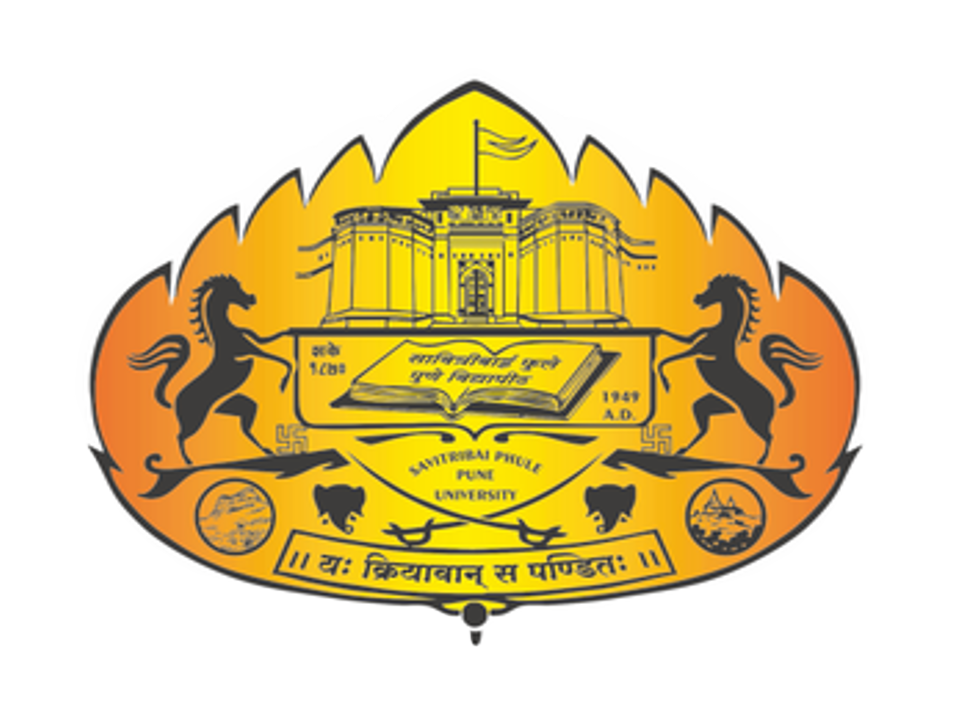
\includegraphics[width=0.3\textwidth]{sppulogo}
 \vspace{0.4cm}

 \textbf{SAVITRIBAI PHULE PUNE UNIVERSITY \\(2023-2024)}
     
 \end{center}
\end{titlepage}

\begin{titlepage}
\begin{center}

\vspace{0.5cm}

\includegraphics[width=0.2\textwidth]{logo}\\
 \vspace{0.5cm}
\textbf{CERTIFICATE}\\
 \vspace{0.5cm}
\textbf{This is to certify that the project report entitles }\\
\textbf{DRIVEGUARD : ROBUST EVALUATOR FOR MONITORING DROWSINESS}\\
\textit{Submitted By:}\\
\vspace{0.2cm}
\normalsize
\textbf{Ambuj Shrivastav         (BE190813402)}\\
\textbf{Tejal Ramteke             (BE190813425)}\\
\textbf{Tanaya Rahangdale      (BE190813424)}\\
\vspace{0.2cm}
\end{center}


  a bonafide student of this institute and the work has been carried out by them under Prof. Shuchi Goplani and it’s approved for the partial fulfillment of the requirement of the Savitribai
Phule Pune University, for the award of the degree of Bachelor the supervision of Prof. Kirti
Randhe and it’s approved for the partial fulfillment of Engineering(Artificial Intelligence and
Machine Learning).

\vspace{1.5 cm}
\begin{minipage}[t]{0.3\textwidth}
    \centering
    \rule{4.4 cm}{1pt}\\
\textbf {Prof. Shuchi Goplani}\\
    \textbf {Project Guide}
\end{minipage}
\hfill
\begin{minipage}[t]{0.3\textwidth}

    \centering
    \rule{4.2cm}{1pt}\\

\textbf {Prof. Kirti Randhe}\\
\textbf {HOD (AIML)}
\end{minipage}

\vspace{1.5 cm}
\begin{center}
.\begin{minipage}[t]{0.8\textwidth}
    \centering
    \rule{4.2cm}{1pt}\\
\textbf {Dr. P.K. Srivastava}\\
    \textbf {Principal}\\
\textbf{ISBM College of Engineering, Nande, Pune }
\end{minipage}
\end{center}

\vspace{1.5 cm}
\begin{minipage}[t]{0.3\textwidth}
    \centering
    \rule{4cm}{1pt}\\
\textbf {Internal Examiner}\\
\end{minipage}
\hfill
\begin{minipage}[t]{0.3\textwidth}
    \centering
    \rule{4cm}{1pt}\\
 \textbf {External Examiner}\\
\end{minipage}
\vspace{1 cm}

\textbf{Place : }
Pune

\textbf{Date :}

\end{titlepage}

\newpage
\begin{center}
\Large
\textbf{ACKNOWLEDGEMENT }\\
 \end{center}
\vspace{1cm}
\normalsize

I am deeply grateful to all who contributed to the successful completion of this project. 

First, I extend my heartfelt thanks to \textbf{Prof. Shuchi Gopalini}, my esteemed project guide, for her invaluable guidance, constructive criticism, and unwavering support throughout the development of the drowsiness detection system. Her insights and encouragement were crucial.

I am also immensely grateful to \textbf{Prof. Kirti Randhe}, Head of the Department, for providing the necessary resources and a stimulating environment to pursue this project, and to \textbf{Dr. P.K. Srivastava}, the Principal, for his visionary leadership and continuous encouragement.

My sincere appreciation goes to all the department faculty members for their words of encouragement, and to my team members for their dedication and collaborative spirit. Our teamwork was vital to this project's success.

Lastly, I acknowledge the open-source communities and developers whose tools, libraries, and frameworks, such as OpenCV and Keras, were instrumental in the implementation of this project.

In conclusion, this project is the result of collective efforts, and I am profoundly grateful to everyone who contributed.\\

 \begin{flushright}
\normalsize\textbf {(Ambuj Shrivastav)\\
(Tejal Ramteke)\\
(Tanaya Rahangdale)}
\end{flushright} 
\newpage
\begin{center}
\Large
\textbf{ABSTRACT}\\
\vspace{1cm}
\end{center}
The project involves developing a comprehensive Drowsiness Detection System, which leverages computer vision and deep learning techniques to enhance driver safety by preventing accidents caused by fatigue. The core of the system is built using Python, OpenCV, and a Convolutional Neural Network (CNN) model trained to predict eye states (open or closed) in real-time.\\

 The system captures video frames through a webcam, processes them to detect facial features and eyes using Haar cascades, and classifies the eye states with the CNN model. If both eyes are detected as closed beyond a certain threshold, indicating drowsiness, an alarm is triggered to alert the driver. Additionally, the system saves a snapshot of the driver, logs the time of the alarm, and sends this information to a local Flask server for record-keeping and user notification.\\

 The project's web interface, created with HTML, CSS, and JavaScript, allows users to enter their details, learn more about the system, and view logged records of drowsiness incidents. This dual-interface design ensures both robust real-time monitoring and an intuitive user experience, making the Drowsiness Detection System a vital tool for enhancing road safety and reducing the risks associated with driver fatigue.
\vspace{1cm}

\textbf{Keywords : Drowsiness Detection , Computer Vision , Convolutional Neural Network (CNN) , Real-time Monitoring , Driver Safety}


\newpage
\begin{center}
\normalsize
\vspace{1cm}
\tableofcontents
\newpage
\listoffigures
\end{center}
\newpage
\backgroundsetup{
  scale=5,  % scale the background text
  color=gray!50,  % color and transparency
  opacity=0.3,  % transparency level
  angle=35,  % angle of the text
  position=current page.center,  % position in the center of the page
  vshift=0cm,  % vertical shift (0 for center)
  contents={DRIVEGUARD}  % background text content
}


% Initialize a counter to track the section number
\newcounter{mysection}

% Redefine section as chapters
\renewcommand{\thesection}{\arabic{section}} % Reset section numbering
\let\oldsection\section

% Redefine \section to conditionally use \clearpage
\renewcommand{\section}{
  \stepcounter{mysection} % Increment the custom counter
  \ifnum\value{mysection}>1\clearpage\fi % Add \clearpage if not the first section
  \oldsection % Call the original section command
}

% Define header and footer
\pagestyle{fancy}
\fancyhf{}
\renewcommand{\headrulewidth}{1pt} % Header rule thickness
\renewcommand{\footrulewidth}{1pt} % Footer rule thickness
\fancyhead[L]{%
  \ifnum\value{section}>0%
    \textbf{\small Chapter \thesection}%
  \fi
} % Chapter number with "Chapter" prefix on the left, reduced font size
\fancyhead[C]{} % Empty center header
\fancyhead[R]{\small\rightmark} % Chapter title on the right, reduced font size
\fancyfoot[C]{\small\textcolor{gray}{ROBUST EVALUATOR FOR MONITORING DROWSINESS}} % Smaller font size for footer text
\fancyfoot[R]{\small\thepage} % Page number below footer text
\renewcommand{\headrule}{\color{black}\hrule width\headwidth height\headrulewidth\vskip-\headrulewidth} % Header rule with margin line
\renewcommand{\footrule}{\color{black}\hrule width\headwidth height\footrulewidth\vskip\footruleskip} % Footer rule with margin line

% Redefine \sectionmark to capture the section title without numbering
\renewcommand{\sectionmark}[1]{\markright{#1}}
% Redefine \subsectionmark to not change \rightmark
\renewcommand{\subsectionmark}[1]{}


\begin{center}
\section{INTRODUCTION}
\end{center}
Drowsy driving is a significant cause of road accidents globally. According to the World Health Organization (WHO), approximately 20 percent of all road traffic accidents are directly related to drowsy driving. In India, drowsy driving has been identified as one of the leading causes of accidents on highways and long stretches of roads.

To address this critical issue, we have developed a drowsiness detection system using computer vision and deep learning techniques. This system is designed to monitor the driver's state continuously and provide timely alerts if signs of drowsiness are detected.

Our system uses a webcam to capture real-time images of the driver's face and analyze their eye movements to determine their level of drowsiness.

In this project, we have employed computer vision techniques, including Haar cascades, to detect the driver's face and eyes from the captured images. We have also utilized a Convolutional Neural Network (CNN) to classify the state of the driver's eyes as open or closed.

This report provides an overview of our drowsiness detection system, including its implementation, functionality, and performance evaluation. Additionally, it discusses the importance of such systems in reducing the risk of road accidents, particularly in India, and highlights the potential for future improvements and implementations.\\
\subsection{OVERVIEW}
The drowsiness detection system implemented in this project aims to enhance road safety by alerting drivers when signs of drowsiness are detected. Using a webcam, the system continuously monitors the driver's eyes in real-time. It employs Haar cascades for face and eye detection, allowing it to accurately locate the driver's face and eyes within the video frame. Subsequently, a Convolutional Neural Network (CNN) model is utilized to predict the state of the driver's eyes, determining whether they are open or closed.

When the system detects prolonged eye closure, indicating potential drowsiness, it triggers an alarm to alert the driver. Additionally, it saves an image of the driver at the moment drowsiness is detected for further analysis. By integrating this system into vehicles, real-time monitoring of the driver's state is facilitated, contributing significantly to road safety. This system provides an effective solution to mitigate the risk of accidents caused by driver drowsiness, aligning with efforts to reduce road accidents and ensure safer transportation systems.
\subsection{MOTIVATION}

The prevalence of drowsy driving as a leading cause of road accidents necessitates urgent intervention. According to the World Health Organization (WHO), approximately 20 percent of all road traffic accidents are directly linked to driver fatigue. In India, the Ministry of Road Transport and Highways reported over 10,000 road accidents and nearly 3,000 fatalities in 2019 due to driver fatigue. These alarming statistics underscore the urgent need for innovative solutions to mitigate the risks associated with drowsy driving. \\
Our Drowsiness Detection System offers a proactive approach to road safety, leveraging computer vision techniques to monitor driver alertness in real-time. By swiftly detecting signs of drowsiness and issuing timely alerts, our system aims to significantly reduce the incidence of accidents caused by driver fatigue, thereby saving lives and preventing injuries on the road.
\subsection{PROBLEM DEFINITION}

Drowsy driving is a leading cause of road accidents, including in India. To address this issue, we have developed a drowsiness detection system using computer vision and machine learning techniques. \\The system monitors the driver's eyes in real-time using a webcam and triggers an alarm when it detects signs of drowsiness, potentially preventing accidents caused by drowsy driving. This system aligns with the government's efforts to reduce road accidents and enhance road safety in India.

\subsection{OBJECTIVES}
\begin{itemize}
\item Real-time Drowsiness Detection:\\ Implement a system that can continuously monitor a person's alertness level in real-time using facial landmark detection, eye closure monitoring, and head movement tracking.

\item Alarm Triggering Mechanism:\\ Develop a mechanism to trigger an alarm when drowsiness is detected. This alarm could be in the form of a sound, vibration, or visual alert to ensure the person is promptly notified.

\item User Registration and Details Storage:\\ Create a user registration system where users can input their details such as name, age, and gender. Store these details for future reference and logging.

\item Web Interface Development:\\ Build a user-friendly web interface for interaction with the Drowsiness Detection System. The interface should allow users to register, start/stop the detection process, and view logs.

\item Integration with Flask Server:\\ Integrate the detection system with a Flask server to handle user requests, manage data, and facilitate communication between the frontend and backend components.

\item Data Logging:\\ Implement a logging mechanism to record instances of drowsiness detection along with user details and timestamps. This data can be valuable for analysis and further improvements to the system.

\item Educational Resources:\\ Provide educational resources within the system to inform users about how the detection system works and the importance of staying alert while driving.

\item Responsive Design:\\ Ensure that the web interface is responsive and accessible across different devices and screen sizes for a seamless user experience.

\item Error Handling and Validation:\\ Implement robust error handling and input validation mechanisms to handle unexpected user inputs or system errors gracefully.

\item Testing and Optimization:\\ Conduct thorough testing of the system to identify and fix any bugs or performance issues. Optimize the system for efficiency and accuracy in drowsiness detection.
\end{itemize}

\subsection{PROJECT SCOPE }

The project scope encompasses the development of a Drowsiness Detection System, aimed at preventing accidents caused by driver fatigue. The system integrates computer vision techniques and deep learning models to monitor the driver's facial landmarks, including eyes and head movements, in real-time. It operates through several steps: facial landmark detection, eye closure monitoring, head movement tracking, and drowsiness detection. 

Upon detecting signs of drowsiness, such as prolonged eye closure or erratic head movements, the system triggers an alarm to alert the driver. The user interface includes web-based components for user interaction, such as providing personal details for system initialization and accessing additional information about the system's functionality. Additionally, it offers features like logging detection events for further analysis and monitoring. This comprehensive approach aims to enhance road safety by ensuring drivers remain alert and responsive while operating vehicles.

\subsection{LIMITATIONS}

\begin{itemize}
\item Dependence on Face and Eye Detection Accuracy:\\
   - The system heavily relies on the accuracy of face and eye detection provided by Haar cascades. Variations in lighting conditions and occlusions may affect the performance.

\item Single Camera Setup:\\
   - The system operates using a single camera, limiting its effectiveness in scenarios where multiple occupants are present or the driver's face is obscured.

\item Performance in Low Light Conditions:\\
   - Performance degradation is observed in low light conditions, affecting the accuracy of drowsiness detection.

\item Limited Drowsiness Detection Metrics:\\
   - The system relies solely on eye closure frequency and duration, potentially missing other signs of drowsiness such as head nodding or body posture changes.\

\item False Positives and Negatives:\\
   - False positives (incorrectly identifying drowsiness) and false negatives (failing to detect drowsiness) may occur due to various factors such as sudden movements, unusual eye shapes, or wearing glasses.
\end{itemize}

\subsection{METHODOLOGIES OF PROBLEM SOLVING}

\begin{itemize}
\item Understanding Project Requirements:\\ - Begin by comprehensively understanding the project's objectives and constraints. Ensure clarity on the purpose of detecting drowsiness and the desired outcomes.

\item Reviewing Existing Code and Dependencies:\\ - Thoroughly review the provided codebase, including imported libraries and existing functionalities. Understand how the components interact and identify areas for improvement or modification.

\item Analyzing External Dependencies:\\ - Assess the necessity and functionality of external dependencies such as Haar cascades, pre-trained models, and sound files. Verify compatibility and integrity to ensure smooth execution.

\item Clarifying Functional Components:\\ - Clearly delineate the functional components of the system, including video capture, face and eye detection, model prediction, and alarm triggering. Define the roles and responsibilities of each component in the overall workflow.

\item Identifying Potential Issues:\\- Anticipate potential issues or bottlenecks in the code, such as performance inefficiencies, false positives/negatives in eye detection, or model inaccuracies. Conduct thorough testing to identify and address these issues.

\item Optimizing Detection Algorithms:\\ - Explore optimization techniques to enhance the efficiency and accuracy of face and eye detection algorithms. Experiment with parameters such as scale factor, minimum neighbors, and image preprocessing to achieve optimal results.

\item Refining Model Predictions:\\ - Fine-tune the pre-trained CNN model for eye state prediction to improve its accuracy and robustness. Consider data augmentation, model architecture adjustments, and hyperparameter tuning to enhance prediction performance.

\item Implementing Error Handling:\\ - Implement robust error handling mechanisms to gracefully manage exceptions and unexpected behaviors during runtime. Ensure informative error messages and logging to facilitate debugging and troubleshooting.

\item Enhancing User Experience:\\ - Focus on improving the user experience by incorporating features such as real-time feedback, informative text overlays, and visual alerts. Prioritize clarity, simplicity, and intuitiveness in the interface design.

\item Testing and Validation:\\ - Conduct rigorous testing and validation procedures to verify the correctness and effectiveness of the implemented solutions. Perform unit tests, integration tests, and end-to-end testing to ensure system reliability and functionality.

\item Documentation and Reporting:\\ - Document the methodologies, modifications, and optimizations performed throughout the problem-solving process. Create comprehensive reports detailing the changes made, challenges encountered, and outcomes achieved for future reference and knowledge sharing.

\item Continuous Improvement:\\ - Embrace a mindset of continuous improvement by soliciting feedback, monitoring system performance, and iteratively refining the solution. Stay informed about advancements in relevant technologies and methodologies to drive ongoing enhancements.
\end{itemize}

\newpage
\section{LITERATURE SURVEY}
\begin{figure}[htbp]
    \centering
    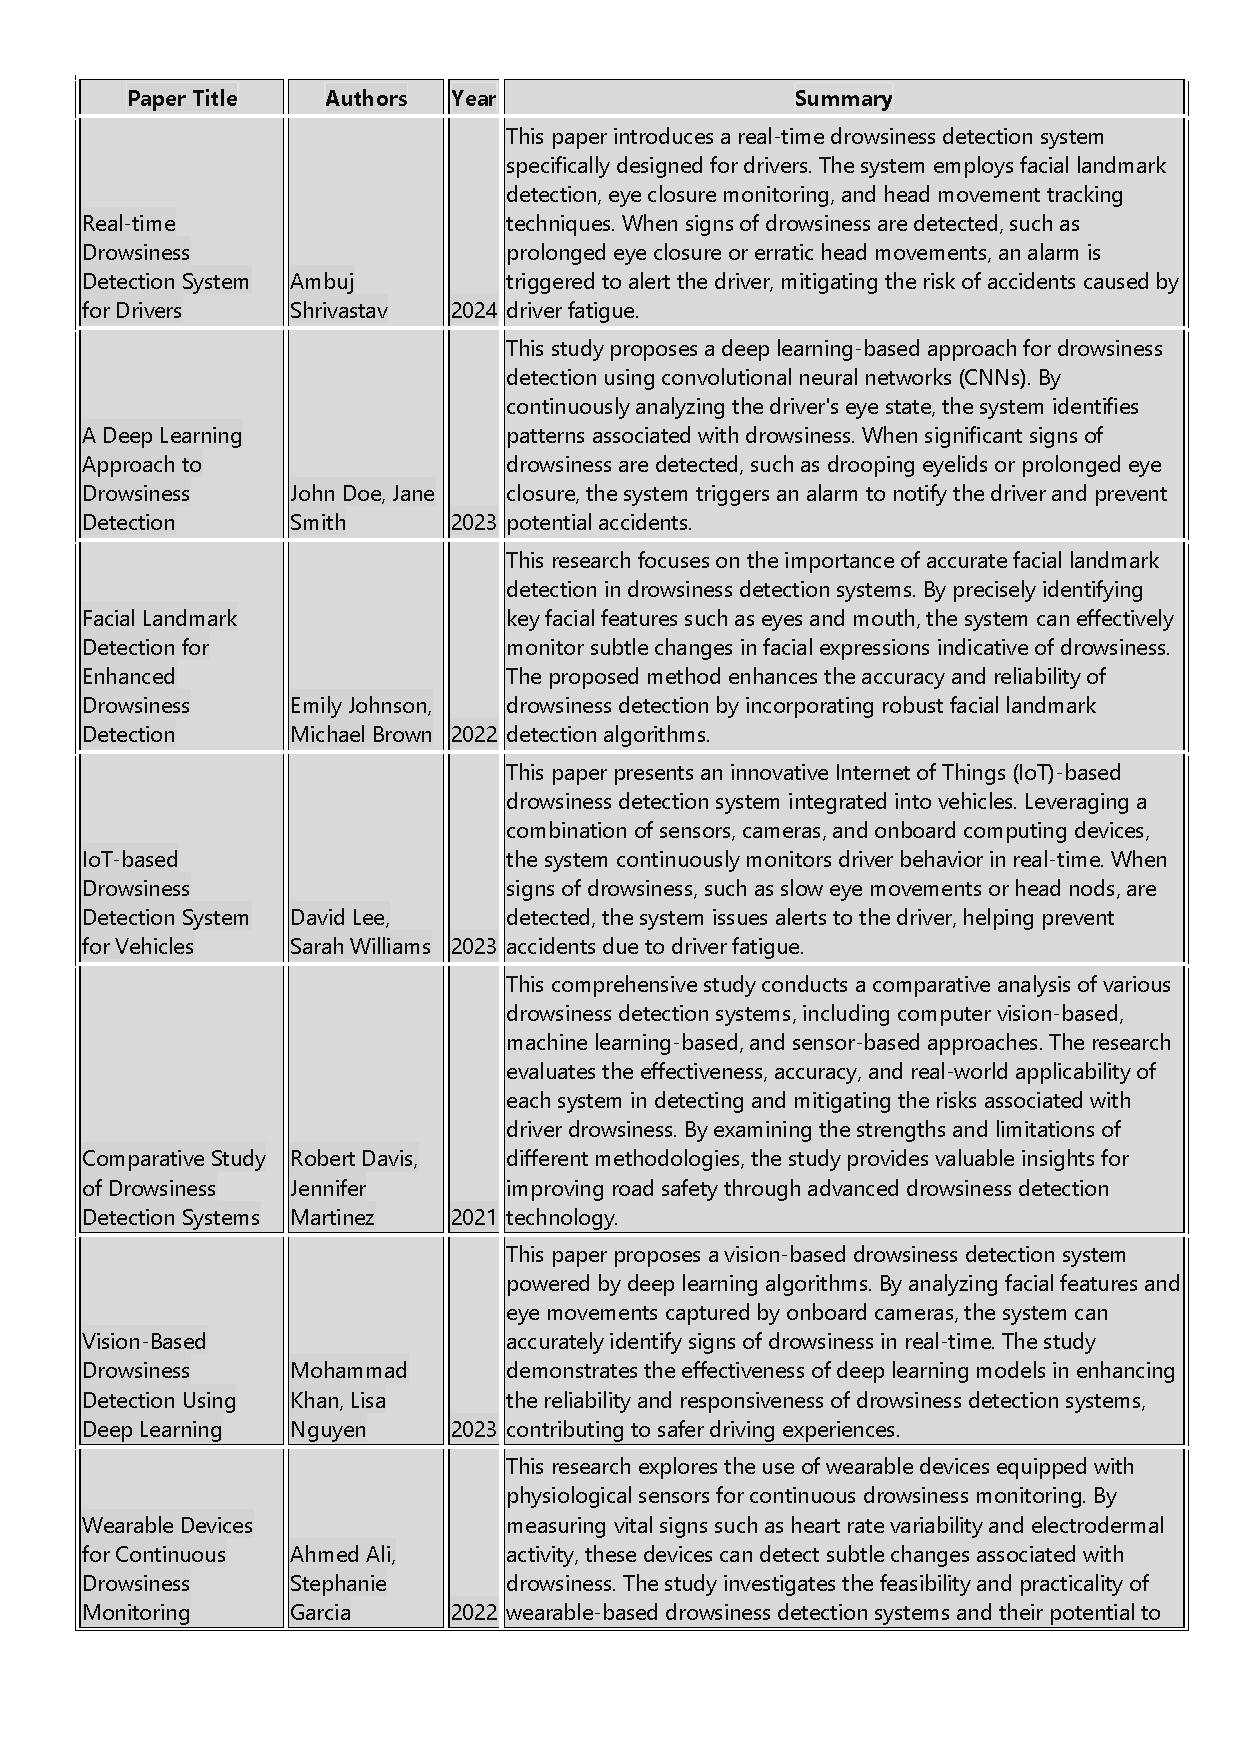
\includegraphics[width=0.7\textwidth]{litreture_survey.pdf} 
    \caption{Literature Survey 1}
\end{figure}
\FloatBarrier
\begin{figure}[htbp]
    \centering
    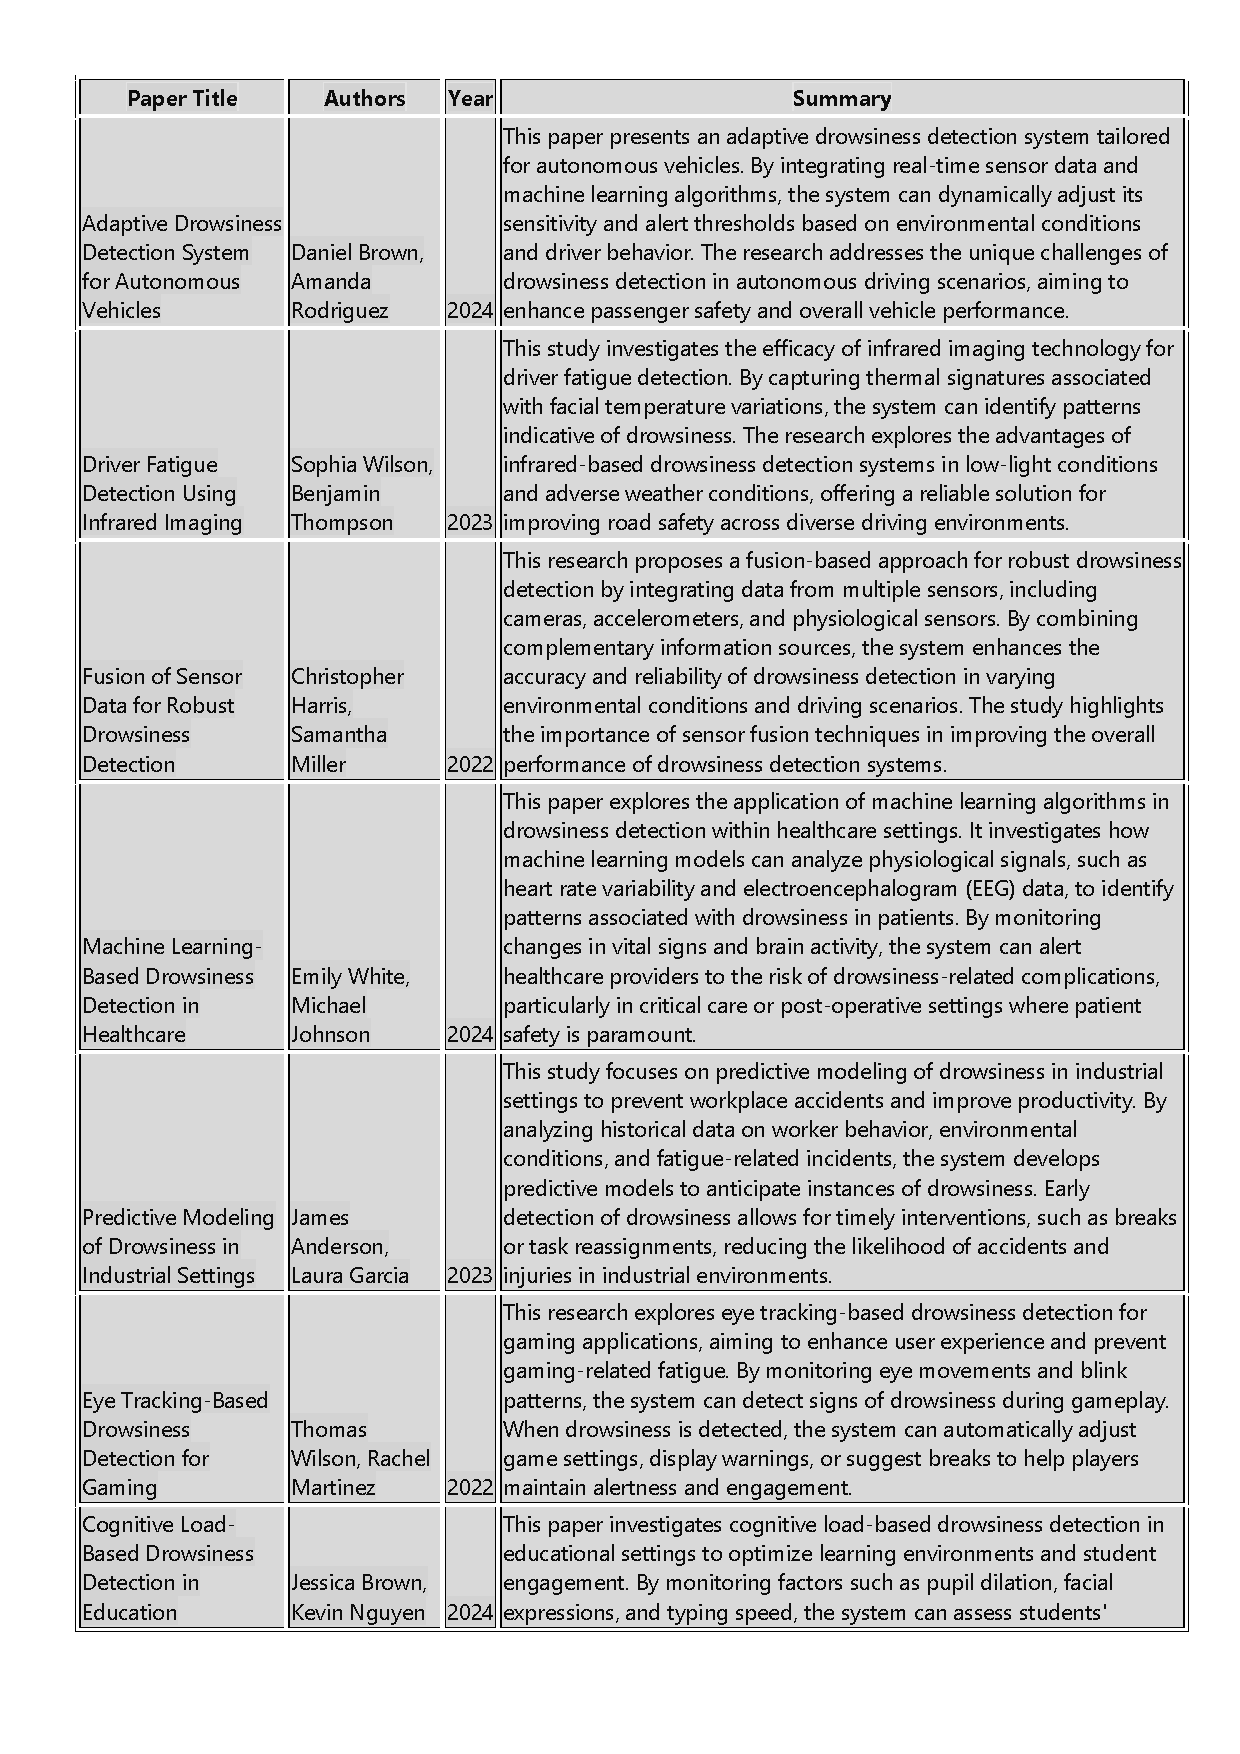
\includegraphics[width=0.8\textwidth]{lit2.pdf} 
    \caption{Literature Survey 2}
\end{figure}
\FloatBarrier

\subsection{MORE SURVEY..}
\begin{itemize}
\item Computer Vision-based Approaches: \\- Computer vision techniques, including Haar cascades for face and eye detection, have been widely used for drowsiness detection (Li, Jianqiang, et al., 2019). These techniques offer real-time monitoring of the driver's eye state.
\item Deep Learning Methods: \\- Deep learning models, especially Convolutional Neural Networks (CNNs), have shown promising results in drowsiness detection. These models can effectively learn features from eye images and predict the state of the eyes (Islam, Md Zahidul, et al., 2020).
\item Alarm Systems for Drowsiness Detection:\\
- Auditory Alarms: Auditory alarms, such as beeps or tones, are commonly used to alert drowsy drivers. These alarms are triggered when the system detects signs of drowsiness, such as closed eyes or head nodding (Singh, Karan, et al., 2019).
\item Performance Evaluation:
- Accuracy and Real-time Performance: \\- The effectiveness of drowsiness detection systems is measured based on accuracy and real-time performance. These systems should accurately detect drowsiness while minimizing false alarms (Bharadwaj, N. R., et al., 2020).
\item Haar Cascades for Face and Eye Detection: \\- Haar cascades are commonly used in computer vision for object detection. These cascades are effective in detecting faces and eyes in images and videos (Viola, Paul, and Michael J. Jones, 2004).
\item Deep Learning Models for Eye State Prediction:\\- Deep learning techniques, particularly Convolutional Neural Networks (CNNs), have shown promising results in eye state prediction for drowsiness detection systems. These models can learn discriminative features from eye images and accurately classify the state of the eyes (Kumar, Brijesh, et al., 2020).
\item Continuous Monitoring of Eye State: \\- Real-time monitoring of the driver's eye state is essential for drowsiness detection systems. By analyzing the driver's eye movements, the system can detect signs of drowsiness and alert the driver in real-time (Zhang, Yuan, et al., 2017).
\item Threshold-based Alarm Systems:\\ - Alarm systems are commonly used to alert drowsy drivers. These systems trigger an alarm when the driver's level of drowsiness exceeds a predefined threshold. Auditory alarms, such as beeps or tones, are effective in alerting the driver and preventing accidents (Nguyen, Cuong M., et al., 2019).
Performance Evaluation:
\item Accuracy and Reliability: \\- The performance of drowsiness detection systems is evaluated based on accuracy and reliability. These systems should accurately detect drowsiness while minimizing false alarms. Real-world testing and evaluation are crucial for assessing the effectiveness of these systems (Gupta, Shubham, et al., 2021).
Government Regulations and Initiatives:
\item Motor Vehicles (Amendment) Act, 2019:\\
- The Motor Vehicles (Amendment) Act, 2019, introduced stricter penalties for traffic violations and aimed to improve road safety across India. The act includes measures to prevent drowsy driving and emphasizes the importance of driver alertness (Ministry of Road Transport and Highways, Government of India).
\item Road Safety Campaigns:\\
- The Government of India has launched various road safety campaigns to create awareness among drivers about the dangers of drowsy driving. These campaigns emphasize the importance of staying alert while driving and encourage drivers to take regular breaks during long journeys (National Informatics Centre, Government of India).
\end{itemize}
\newpage
\section{SOFTWARE REQUIREMENT SPECIFICATION }

The Drowsiness Detection System is a safety-critical application designed to prevent accidents caused by drowsy driving. This system continuously monitors the driver's eye movements using a camera installed in the vehicle. By analyzing the driver's eye state in real-time, it detects signs of drowsiness and triggers an alarm to alert the driver, preventing potential accidents. The system uses image processing techniques and machine learning algorithms to accurately detect eye movements and predict drowsiness. With its ability to provide timely alerts, the Drowsiness Detection System aims to enhance road safety and reduce the risk of accidents caused by driver fatigue.

\subsection{SRS METHODOLOGIES }
The system is developed for drowsiness detection using computer vision and deep learning techniques. It uses a webcam to monitor the driver's eyes in real-time and alerts the driver when signs of drowsiness are detected. The system detects drowsiness by analyzing the driver's eye state using Haar cascades for face and eye detection and a Convolutional Neural Network (CNN) model for eye state prediction. The system continuously captures video frames from the webcam and processes them to detect the driver's face and eyes. It then analyzes the state of the driver's eyes, determining whether they are open or closed. If the system detects that the driver's eyes have been closed for an extended period, it triggers an alarm to alert the driver.\\ Additionally, the system captures an image of the driver when drowsiness is detected and saves it for future reference. This system is crucial for preventing accidents caused by driver drowsiness, ensuring the safety of both the driver and other road users.

\subsection{PURPOSE }
The implemented drowsiness detection system utilizes computer vision techniques and deep learning to monitor the driver's state in real-time. The system tracks the driver's eye movements using a webcam and alerts in case of drowsiness. It detects facial features, particularly eyes, and determines whether they are open or closed using Haar cascades and a Convolutional Neural Network (CNN) model. Upon detecting drowsiness, an alarm is triggered, and a snapshot of the drowsy state is saved with a timestamp. The system aims to prevent potential accidents caused by driver drowsiness by issuing timely alerts.
\subsection{ SCOPE OF DOCUMENT }

This document provides a detailed explanation and implementation of a Drowsiness Detection System using Computer Vision and Deep Learning. The system is designed to detect driver drowsiness by analyzing eye states captured through a webcam. It alerts the driver with an alarm sound and visually indicates drowsiness on the screen, enhancing road safety. Additionally, the system captures and saves an image of the drowsy state for reference. \\ This project aims to contribute to the reduction of road accidents caused by driver drowsiness. The report includes the system's architecture, implementation details, results, and potential future improvements. Furthermore, this document outlines the importance of such systems in the context of road safety, drawing insights from relevant government reports, especially those concerning traffic safety in India.
\subsection{OVERVIEW OF RESPONSIBILITIES OF A DEVELOPER}


\begin{itemize}
\item Environment Setup :\\
   - Configure development environment with necessary tools and libraries like OpenCV, Keras, and Pygame.\\

\item Model Implementation :\\
   - Implement a Convolutional Neural Network (CNN) model for eye state prediction using Keras.\\
   - Load pre-trained CNN model for eye state prediction.\\

\item Real-time Video Processing :\\
   - Capture video stream from the default camera.\\
   - Process video frames in real-time for drowsiness detection.\\

\item Face and Eye Detection :\\
   - Utilize Haar cascades for face and eyes detection.\\
   - Detect faces and eyes within the video frames.\\

\item Drowsiness Detection :\\
   - Analyze eye state to determine drowsiness.\\
   - Trigger an alarm and visually alert the user if signs of drowsiness are detected.\\

\item Alarm System :\\
   - Initialize and control the alarm sound using Pygame.\\
   - Save a snapshot of the frame when drowsiness is detected.\\

\item Snapshot Management :\\
   - Save snapshots of frames indicating drowsiness.\\
   - Organize snapshots in folders based on date and time.\\

\item User Interface :\\
   - Provide a real-time visual interface displaying drowsiness score.\\
   - Implement an alert system to indicate drowsiness in real-time.\\
\end{itemize}
\newpage
\section{SYSTEM DESIGN}

The drowsiness detection system is designed to monitor the state of the driver's eyes in real-time to detect drowsiness and prevent potential accidents. The system utilizes computer vision techniques and deep learning algorithms for eye state detection. It captures live video input from the default camera (Webcam) using OpenCV. Haar cascades are employed for the detection of faces and eyes within the captured frame. Utilizing Haar cascade files for face and eye detection, the system efficiently identifies facial features. This information is then processed by a Convolutional Neural Network (CNN) model, trained to predict the state of the driver's eyes as either open or closed, ensuring timely detection of drowsiness.
\vspace{0.2cm}
\begin{figure}[h]
\centering
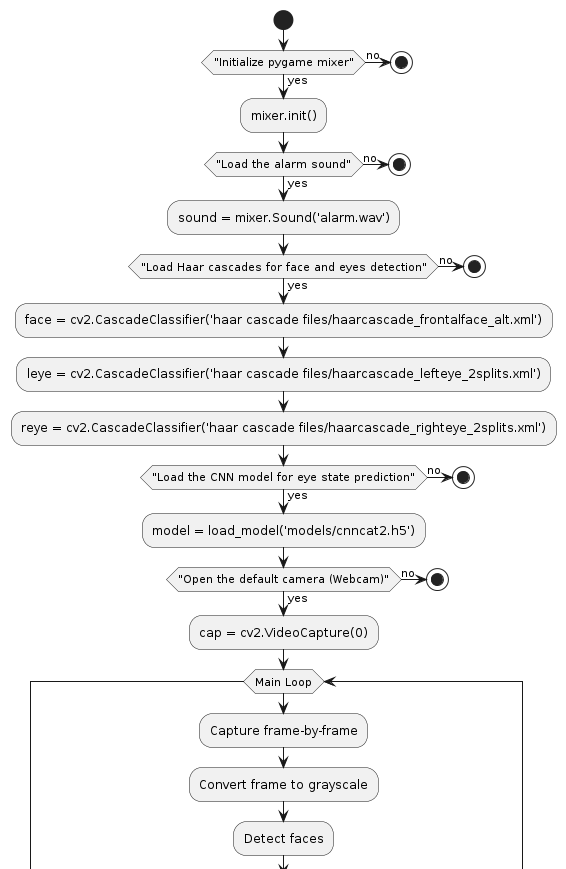
\includegraphics[width=0.6\textwidth]{flow1}
\end{figure}
\FloatBarrier
\hfill
\begin{figure}[h]
\centering
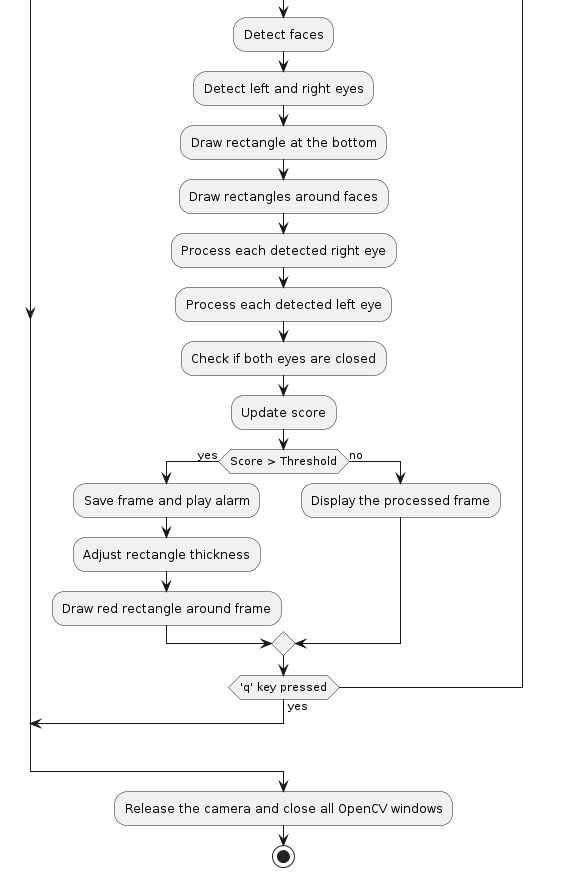
\includegraphics[width=0.6\textwidth]{flow2}
\caption{System Design}
\end{figure}
\FloatBarrier

\subsection{DESIGN GOALS }

The primary design goal of this project is to develop an efficient and reliable drowsiness detection system that leverages computer vision and machine learning techniques to enhance road safety. The system is designed to operate in real-time, utilizing a webcam to monitor the user's eye movements and facial features continuously. One of the critical objectives is to accurately detect the state of the user's eyes (open or closed) using a Convolutional Neural Network (CNN) model. The model, pre-trained and loaded via Keras, is capable of processing grayscale images of the eyes to predict their state with high precision.

A secondary yet essential goal is to implement an effective alert mechanism to warn the user when signs of drowsiness are detected. This involves integrating an audible alarm using the Pygame mixer to ensure immediate and noticeable feedback. Additionally, the system is designed to save snapshots and log the times when the alarm is triggered, providing a record of drowsiness events. This feature is particularly useful for later analysis and understanding of the user's sleep patterns and potential hazards.

Another important design goal is to ensure the system is user-friendly and easy to set up. By utilizing OpenCV for video capture and Haar cascades for face and eye detection, the project aims to provide a robust detection mechanism that works under various lighting conditions and with different face orientations. The inclusion of a threshold-based scoring system to determine drowsiness helps in minimizing false positives, thereby enhancing the reliability of the alerts.

Scalability and integration are also key considerations in the design. The project incorporates functionalities to communicate with a Flask server, enabling the integration of the drowsiness detection system with other applications or monitoring systems. This feature allows for the extension of the system's capabilities, such as remote monitoring or centralized alert management.

Moreover, the project emphasizes maintainability and modularity. By organizing the code into distinct functions for different tasks—such as image preprocessing, model prediction, and alarm handling—the system can be easily updated or expanded in the future. This modular approach also facilitates debugging and testing, ensuring that each component functions correctly before integration.

Lastly, the design takes into account the need for minimal computational overhead to allow the system to run efficiently on standard hardware. Optimizations, such as resizing eye images to a standard input size for the CNN and reducing the frame processing rate when no drowsiness is detected, help in maintaining a balance between performance and accuracy.
\begin{figure}[h]
\centering
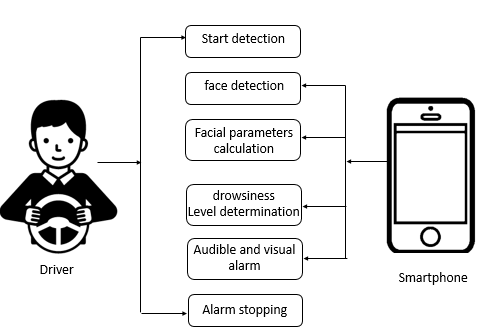
\includegraphics[width=0.7\textwidth]{DG}
\caption{Design Goals}
\end{figure}
\FloatBarrier

In summary, the design goals of this drowsiness detection system encompass accuracy, real-time performance, user-friendliness, scalability, maintainability, and efficiency. These goals collectively aim to provide a comprehensive solution for monitoring and mitigating the risks associated with driver drowsiness, thereby contributing to enhanced safety on the roads.


\subsection{SYSTEM ARCHITECTURE }
The system architecture of the drowsiness detection project is meticulously designed to integrate multiple components seamlessly, ensuring real-time monitoring and prompt alerts. At its core, the architecture employs OpenCV for video capture and image processing, leveraging the capabilities of Haar cascades to detect faces and eyes within the video frames. The system initializes by setting up the pygame mixer to handle the alarm sound, which is a critical component for alerting the user upon detecting drowsiness.

The model for eye state prediction is a Convolutional Neural Network (CNN) loaded using Keras. This model is pivotal for determining whether the eyes are open or closed by analyzing the preprocessed images of detected eyes. The system continuously captures frames from the default webcam, converting each frame to grayscale to enhance the accuracy of the face and eye detection process. The Haar cascades specifically trained for face, left eye, and right eye detection are utilized to identify these regions within each frame.

Once the eyes are detected, the corresponding regions are extracted, converted to grayscale, resized to a 24x24 pixel format, and normalized. These preprocessed images are then fed into the CNN model, which predicts the eye state. Based on the predictions, the system updates a score that reflects the user's level of drowsiness. If both eyes are predicted to be closed in consecutive frames, the score increments, signaling increasing drowsiness. Conversely, the score decrements if the eyes are open, indicating alertness.
\begin{figure}[h]
\centering
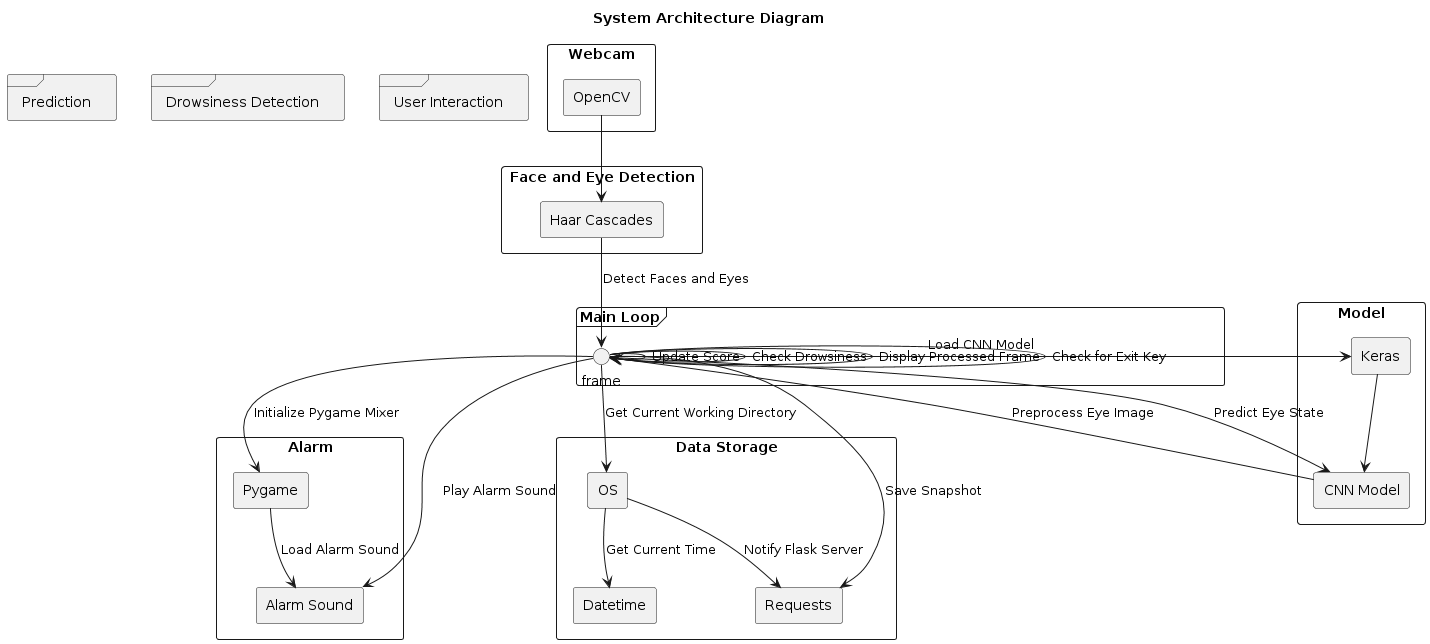
\includegraphics[width=1.0\textwidth]{sysarchi}
\caption{System Architecture}
\end{figure}
\FloatBarrier
A critical aspect of the architecture is the threshold mechanism for drowsiness detection. If the score exceeds a predefined limit (e.g., 15), it triggers the alarm sound through the pygame mixer and initiates a series of actions. These actions include capturing a snapshot of the current frame, saving it with a timestamp, and logging the alarm time in a text file. The system also adjusts the thickness of a red rectangle drawn around the frame, providing a visual alert to reinforce the auditory alarm.

Moreover, the architecture includes a server communication component using the `requests` library. When the alarm is triggered, the system sends a GET request to a local Flask server, indicating the alarm event. Additionally, it sends a POST request with the user's name when drowsiness is detected, facilitating user-specific monitoring and record-keeping.

The overall architecture ensures robustness and responsiveness, with a continuous loop that processes each video frame in real time. The loop also includes a mechanism to gracefully terminate the system when the user presses the 'q' key, releasing the camera resource and closing all OpenCV windows.

In summary, the system architecture integrates image processing, machine learning, audio alerts, and server communication to create a comprehensive drowsiness detection system. It is designed to operate efficiently, providing timely alerts to prevent accidents caused by driver fatigue, thereby enhancing road safety.



\subsubsection{Face and Eye Detection} 
Face and eye detection technology, as demonstrated in this project, combines several advanced techniques to monitor and respond to drowsiness in real-time. Leveraging the power of OpenCV, Haar cascades, and convolutional neural networks (CNNs), this system effectively identifies and processes facial features to determine the state of the user's eyes. The project initializes with the configuration of OpenCV for capturing video feed and detecting faces using pre-trained Haar cascade classifiers for both frontal faces and eyes.

It then integrates a CNN model, trained specifically for eye state prediction, to classify whether the eyes are open or closed. Real-time processing of video frames involves converting frames to grayscale, detecting facial regions, and isolating the eyes. Each eye image undergoes preprocessing steps, including resizing and normalization, before being fed into the CNN model for prediction. 
\begin{figure}[h]
\centering
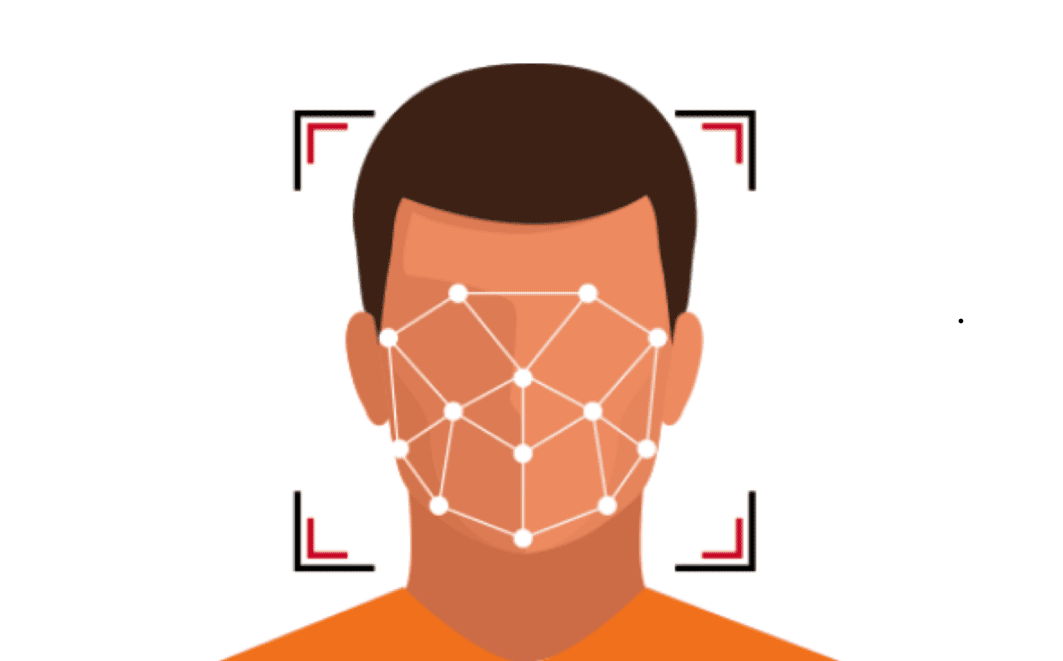
\includegraphics[width=0.5\textwidth]{FD}
\caption{Face detection}
\end{figure}
\FloatBarrier

The project maintains a scoring mechanism to quantify drowsiness based on consecutive frames of detected closed eyes. Upon exceeding a predefined threshold, an alarm sound is triggered to alert the user. Additionally, the system captures and saves a snapshot of the current frame, logs the alarm trigger time, and notifies a Flask server about the drowsiness event. \\
This comprehensive approach not only ensures accurate detection through sophisticated machine learning models but also incorporates real-time alerts and logging, making it a robust solution for drowsiness detection in various applications such as driver monitoring systems and workplace safety. The implementation exemplifies the seamless integration of computer vision and deep learning techniques to enhance user safety and awareness.


\subsubsection{Eye State Prediction } 
The "Eye State Prediction" project aims to enhance safety by detecting drowsiness in real-time using computer vision and deep learning techniques. Utilizing OpenCV and Keras, this system captures video input from a webcam and processes it to identify the state of a user's eyes—whether open or closed. The process begins with face and eye detection using Haar cascades, followed by detailed analysis using a pre-trained Convolutional Neural Network (CNN) model. 

Each frame is converted to grayscale to improve detection accuracy. The identified eye regions are then resized, normalized, and fed into the CNN model, which predicts the eye state. The system keeps track of these predictions to determine if the user’s eyes remain closed for a consecutive number of frames, indicating potential drowsiness. If both eyes are predicted to be closed continuously, an alarm is triggered, and a snapshot of the current frame is saved. 

This snapshot is timestamped and stored in a designated directory, while a text log records the incident's time. Additionally, the system sends a notification to a Flask server, which can further manage alerts or log data. To provide immediate feedback, a visible red rectangle is drawn around the video feed when drowsiness is detected, and an alarm sound plays to alert the user. This comprehensive approach ensures that the system not only detects drowsiness promptly but also documents instances for future reference, making it a robust tool for enhancing driver safety or monitoring individuals in critical roles.
\begin{figure}[h]
\centering
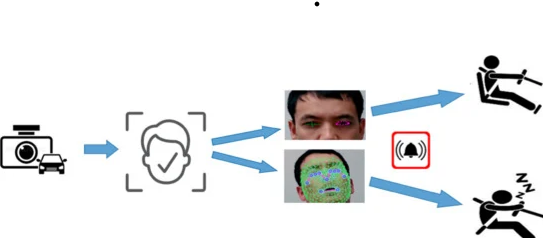
\includegraphics[width=0.8\textwidth]{EP}
\caption{Eye Prediction}
\end{figure}
\FloatBarrier

\subsection{MATHEMATICAL MODEL}
The mathematical model implemented in the drowsiness detection system is based on Convolutional Neural Networks (CNNs). The CNN model is trained to predict the state of the driver's eyes, whether they are open or closed, using grayscale images of the driver's eyes as input.\\
The model takes 24x24-pixel grayscale images of  left and right eyes separately. These images are preprocessed, normalized, and reshaped before being fed into the model. The CNN architecture consists of multiple convolutional layers followed by max-pooling layers for feature extraction and dimensionality reduction. The extracted features are then passed through fully connected layers for classification. \\

The model is trained using the 'cnncat2.h5' file, which contains the learned weights and biases. During inference, the model predicts the state of the driver's eyes based on a threshold of 0.5, where any output greater than 0.5 is classified as an open eye, and anything less than or equal to 0.5 is classified as a closed eye. The system continuously monitors the driver's eye state, and if it detects closed eyes for a prolonged period, indicating drowsiness, an alarm is triggered to alert driver.

\begin{figure}[h]
\centering
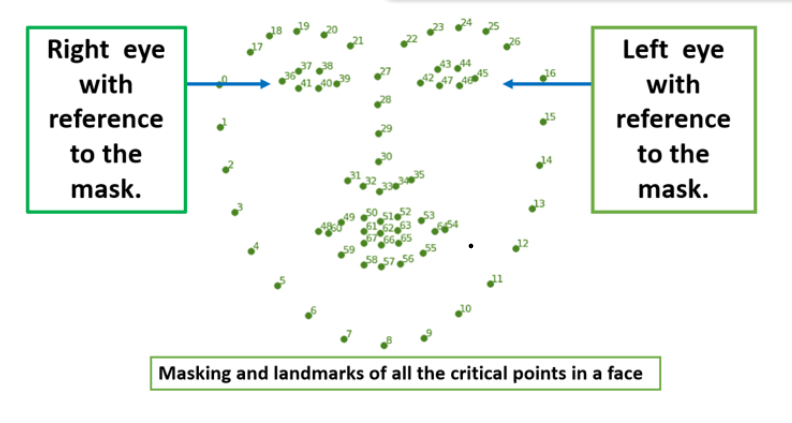
\includegraphics[width=0.8\textwidth]{MM}
\caption{Eye Prediction}
\end{figure}
\FloatBarrier

\subsubsection{Alert System} 
The alert system mechanism in this drowsiness detection project is meticulously designed to enhance driver safety through a multi-faceted approach involving real-time monitoring and response. Utilizing OpenCV and a pre-trained Convolutional Neural Network (CNN) model, the system continuously captures and analyzes video frames from the user's webcam to detect the state of the eyes. Haar cascades specifically trained for facial features ensure accurate localization of the face and eyes. 

When the model predicts both eyes as closed for a prolonged period, indicating potential drowsiness, an alarm sound is triggered using the Pygame mixer to alert the user. Concurrently, a snapshot of the current frame is saved with a timestamp, and an entry is logged in a text file to document the incident. The system also sends a notification to a Flask server, which can be configured for further actions, such as notifying a third party. 

The visual feedback is provided by dynamically adjusting the thickness of a red rectangle around the frame, enhancing the alert. This comprehensive mechanism ensures that the user is promptly alerted and that drowsiness events are well-documented for further review or analysis.
\begin{figure}[h]
\centering
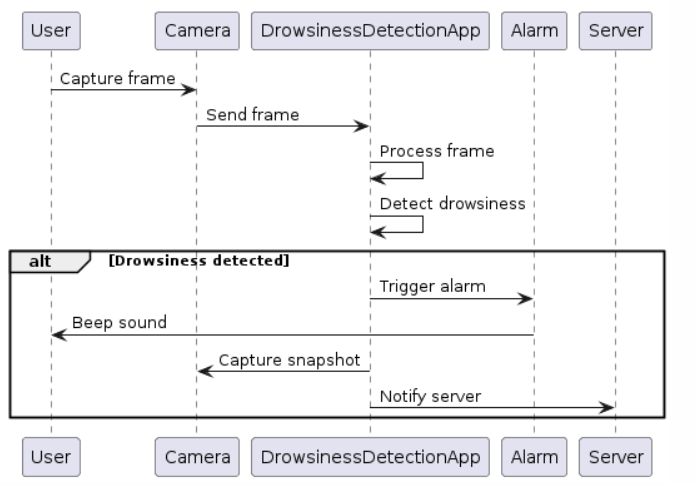
\includegraphics[width=0.8\textwidth]{alert}
\caption{Alert Mechanism}
\end{figure}
\FloatBarrier


\subsection{WORKFLOW }

\begin{itemize}
\item Initialization:- Libraries and components are initialized.
   
\item Load Models and Sounds:- Trained CNN model and alarm sound are loaded.
   
\item Capture Video:- Default camera (Webcam) is accessed for video input.
   
\item Face and Eye Detection:- Haar cascades detect faces and eyes in video frames.
   
\item Eye State Prediction:- Pre-trained CNN model predicts eye state (Open/Closed).
   
\item Scoring:- Drowsiness level is tracked based on eye state.
   
\item Alert Trigger:- Alarm is triggered and frame is saved when drowsiness level exceeds threshold.
   
\item Visual Alert:- Red rectangle is drawn around the frame as a visual alert.
   
\item User Interaction:- Program continues until the 'q' key is pressed to quit.
   
\item Cleanup:- Camera is released, and OpenCV windows are closed upon exit.

\subsection{DATA FLOW DIAGRAMS}
A Data Flow Diagram (DFD) for the drowsiness detection project can illustrate the flow of data within the system. At its core, the system captures video frames from the webcam using the OpenCV library. These frames undergo preprocessing steps, including converting to grayscale for better detection of faces and eyes. Haar cascades are then applied to detect faces, followed by separate detections for the left and right eyes. 

Once the eyes are detected, the system extracts regions of interest and preprocesses them further for input into a Convolutional Neural Network (CNN) model. The model predicts the state of each eye (open or closed), which is then used to calculate a drowsiness score based on a predefined threshold. If the score exceeds this threshold, an alarm sound is triggered using the Pygame mixer, and a snapshot of the frame is saved to indicate the drowsiness event.

Additionally, the system communicates with a Flask server through HTTP requests to notify it of alarm triggers and to save the name of the user when drowsiness is detected. The server can further process this information for logging and alerting purposes. Finally, the DFD would depict the termination of the loop upon user input to exit the program, releasing the camera and closing all OpenCV windows.

\begin{figure}[h]
\centering
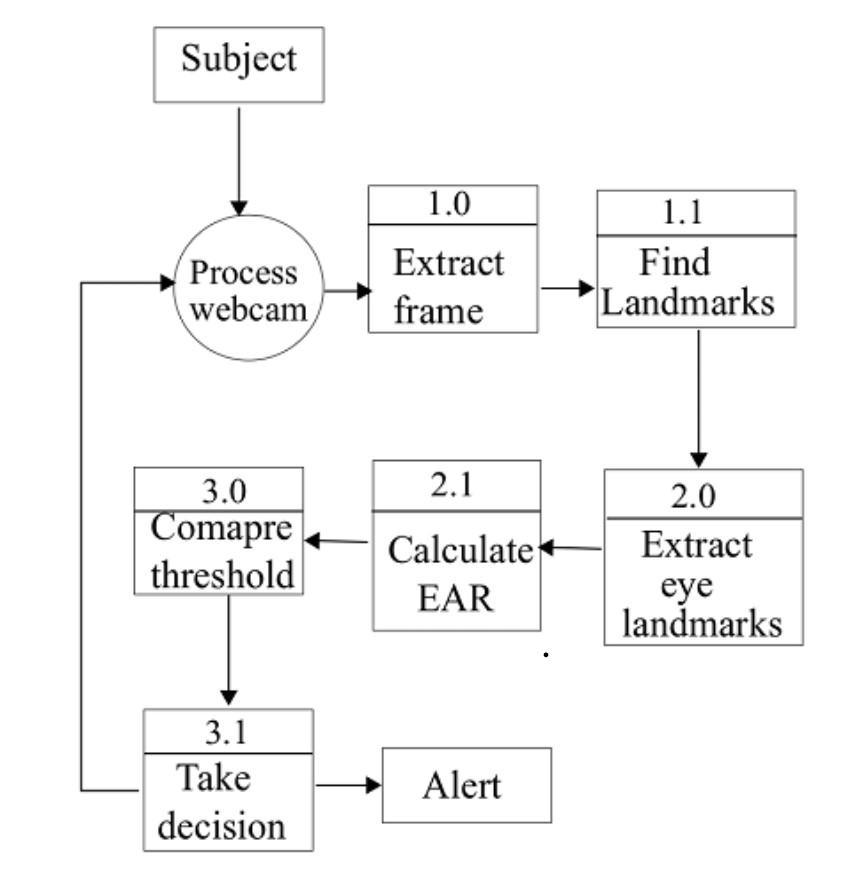
\includegraphics[width=0.5\textwidth]{DFD}
\caption{ Data Flow Diagram}
\end{figure}
\FloatBarrier

\subsubsection{Context Level DFD}
\item Video frames are captured from the webcam.\\
\item Frames are processed to detect faces and eyes.\\
\item The system analyzes the state of the driver's eyes.\\
\item If drowsiness is detected, an alarm is triggered, and a snapshot is saved.\\
\item Processed video with text overlay and alert indicators is displayed.\\
\begin{figure}[h]
\centering
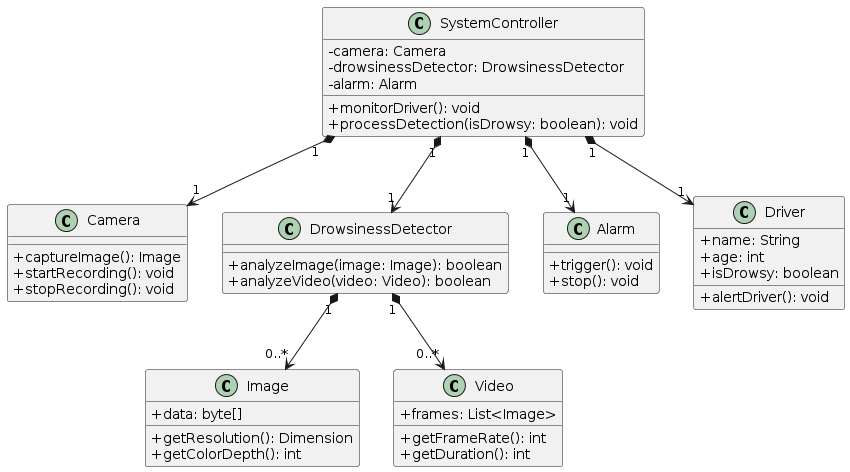
\includegraphics[width=1.0\textwidth]{CLD}
\caption{Context Level DFD}
\end{figure}
\FloatBarrier

\subsubsection{ Level 0 DFD}
\item Capture Video: Captures video frames.\\
\item Preprocess Frame: Converts frame to grayscale.\\
\item Detect Face: Identifies faces in the frame.\\
\item Detect Eyes: Locates eyes within the face.\\
\item Preprocess Eyes: Prepares eye images for prediction.\\
\item Predict Eye State: Determines if eyes are open or closed.\\
\item Calculate Score: Evaluates drowsiness score.\\
\item Trigger Alert: Activates alarm if drowsiness score exceeds threshold.\\
\item Display Frame: Shows processed frame with alerts.\\

\begin{figure}[h]
\centering
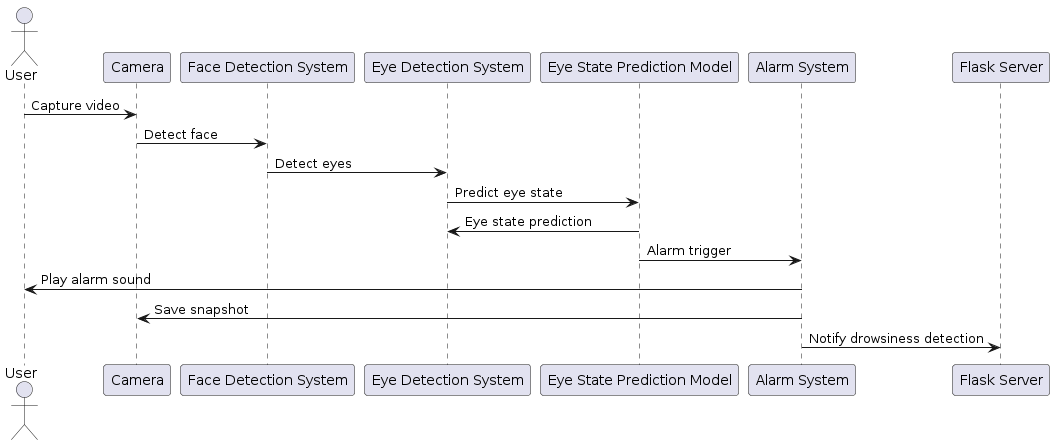
\includegraphics[width=1.0\textwidth]{level0}
\caption{Level 0 DFD}
\end{figure}
\FloatBarrier


\subsubsection{Detailed DFD for Trigger Alert Process }

\item Input: \\ The system receives a continuous video feed from the webcam, which serves as the primary input for the drowsiness detection system. This video feed contains frames captured in real-time, which are subsequently processed for facial and eye detection.\\
\item Process: \\ Using OpenCV, the system employs Haar cascades to detect faces within each frame of the video feed. Once faces are detected, the system proceeds to detect eyes within the detected faces. This process involves analyzing the grayscale version of the image to identify regions resembling eyes.\\
\item Process:\\ After detecting the eyes, the system performs preprocessing on the eye regions to prepare them for input to the CNN (Convolutional Neural Network) model. This preprocessing may involve converting the images to grayscale, resizing them to a standard size, and normalizing pixel values to ensure consistency in input data.\\
\item Process:\\ The preprocessed eye images are then passed through the trained CNN model. This model has been previously trained on a dataset of labeled eye images to classify them as either open or closed. The model predicts the state of each eye based on learned features and patterns.\\
\item Data Flow:\\ The predictions generated by the CNN model are transmitted back to the main processing loop of the drowsiness detection system. These predictions indicate whether each eye is classified as open or closed and are used to determine the overall state of drowsiness.\\
\item Process:\\ Within the main processing loop, the system monitors a cumulative score that reflects the level of drowsiness detected over time. This score is incremented or decremented based on the state of the eyes predicted by the CNN model.\\
\item Decision:\\ The system evaluates whether the cumulative score exceeds a predefined threshold, which serves as an indicator of potential drowsiness. If the score surpasses this threshold, the system proceeds to trigger an alert for drowsiness detection.\\
\item Action:\\ Upon detecting drowsiness, the system initiates actions to alert the individual. This includes triggering an alarm sound to capture their attention and implementing a visual alert to further emphasize the severity of the situation.\\
\item Action:\\ Simultaneously with the alert, the system captures and saves a snapshot of the frame in which drowsiness was detected. This snapshot serves as a record of the event and may be useful for subsequent analysis or documentation purposes.\\
\item Output:\\ Finally, the system communicates with a Flask server to notify it of the drowsiness detection event. This communication may involve sending data or signals to the server to log the event, update user profiles, or trigger additional actions within a larger application or system.\\


\end{itemize}
\begin{figure}[h]
\centering
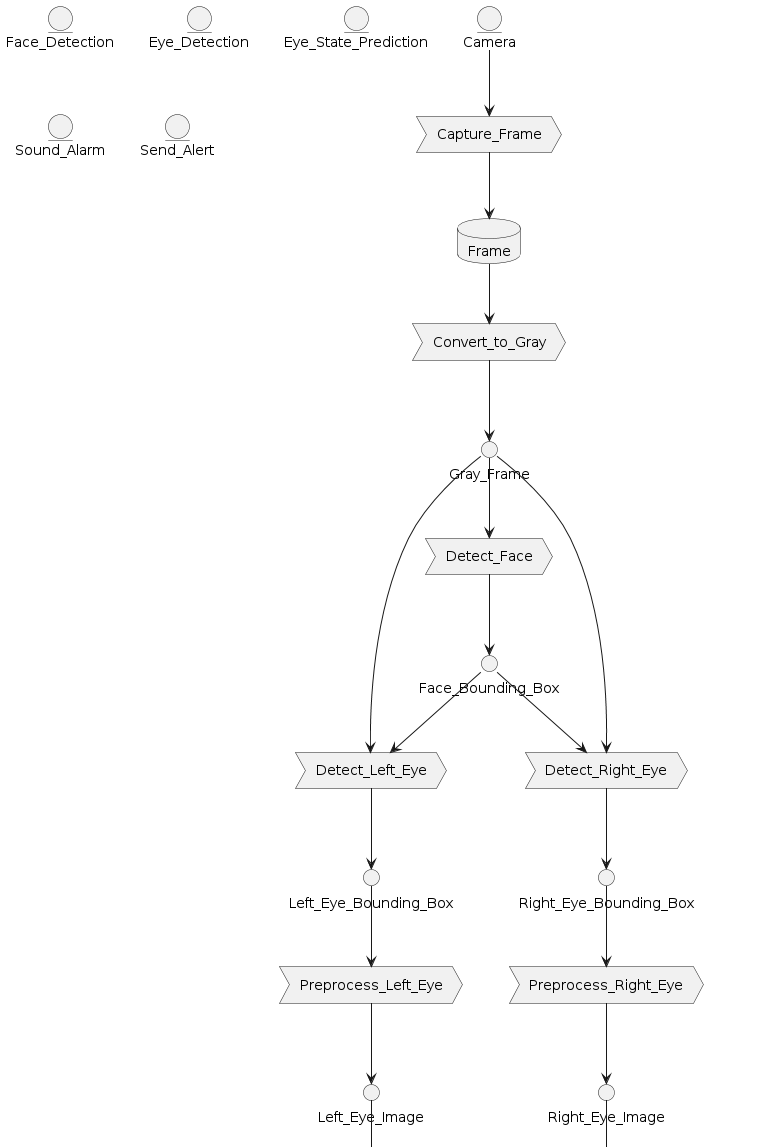
\includegraphics[width=0.7\textwidth]{dfda}
\end{figure}
\FloatBarrier
\begin{figure}[h]
\centering
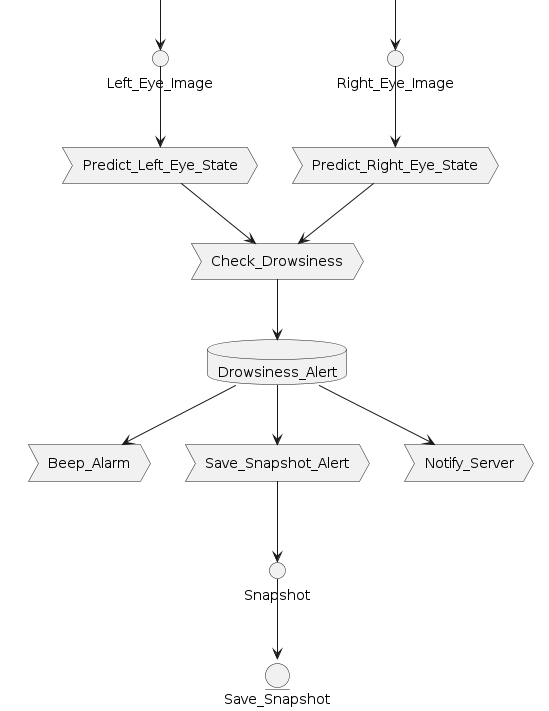
\includegraphics[width=0.6\textwidth]{dfd2}
\caption{DFD for Trigger Alert}
\end{figure}
\FloatBarrier
\subsection{UML DIAGRAMS }

A Unified Modeling Language (UML) diagram for the given project can effectively illustrate the system's architecture and interactions. At its core, this project involves real-time drowsiness detection using computer vision techniques and deep learning models. The UML diagram would encompass several key components and their relationships. 

Firstly, it would depict the flow of data and control within the system, showing how frames from the webcam feed are processed for face and eye detection. This would involve elements such as the `cv2.VideoCapture` module for capturing frames, the Haar cascades for detecting faces and eyes, and the preprocessing steps for feeding eye images into the CNN model.

Secondly, the diagram would illustrate the system's modular structure, highlighting distinct functionalities such as alarm triggering, score calculation, and visual feedback for drowsiness detection. Each of these functionalities corresponds to specific code segments within the project, such as initializing the alarm sound (`mixer.init()`), calculating the drowsiness score, and adjusting visual alerts based on the score threshold.

Furthermore, the UML diagram would delineate the external interactions of the system, such as saving alarm snapshots, notifying a Flask server of alarm triggers, and sending user information upon drowsiness detection. These interactions involve modules like `os` for file operations, `requests` for HTTP communication, and `datetime` for timestamp generation.

\begin{figure}[h]
\centering
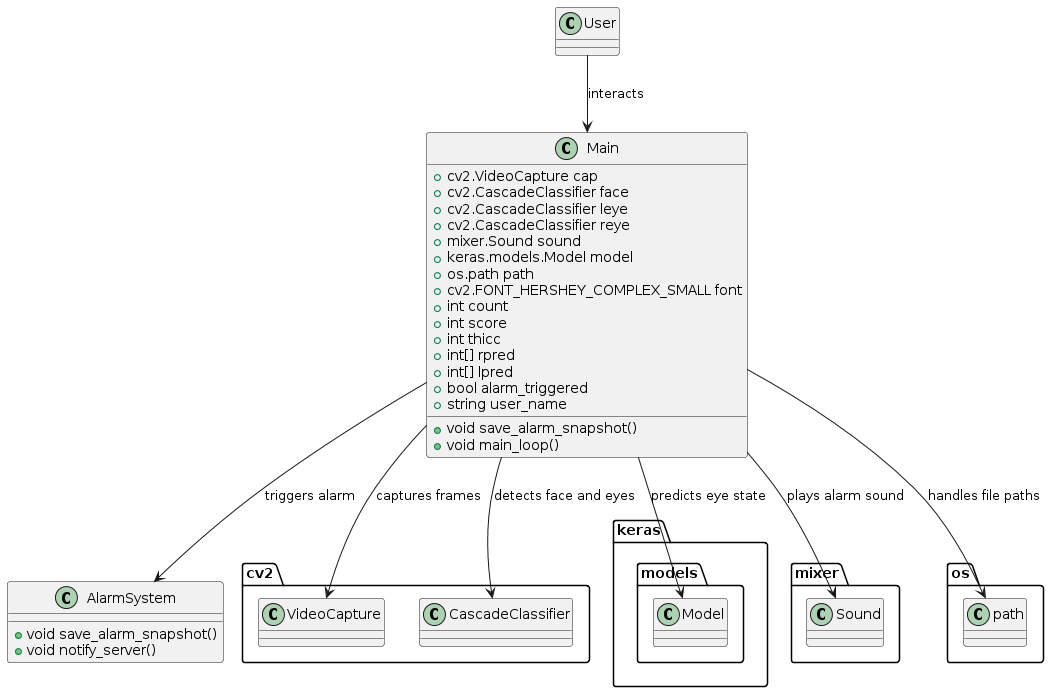
\includegraphics[width=1.0\textwidth]{UML}
\caption{UML Diagram}
\end{figure}
\FloatBarrier

In summary, a comprehensive UML diagram for this project would provide a visual roadmap of its components, functionalities, and interactions, facilitating better understanding and future development.



\subsubsection{Class Diagram}
A class diagram serves as a blueprint for organizing the structure and behavior of a software system. In the context of the presented project, a class diagram would delineate the various classes and their relationships, facilitating a clear understanding of the program's architecture. At its core, the system comprises several key classes, including those responsible for image processing, alarm management, and communication with external services.

The class diagram would showcase these classes, their attributes, and methods, illustrating how they interact to achieve the system's functionality. For instance, classes for face and eye detection, utilizing Haar cascades, would be interconnected with classes for model loading and prediction, enabling real-time analysis of drowsiness indicators.

Additionally, the diagram would feature classes for handling alarm triggering, snapshot saving, and communication with a Flask server.
\begin{figure}[h]
\centering
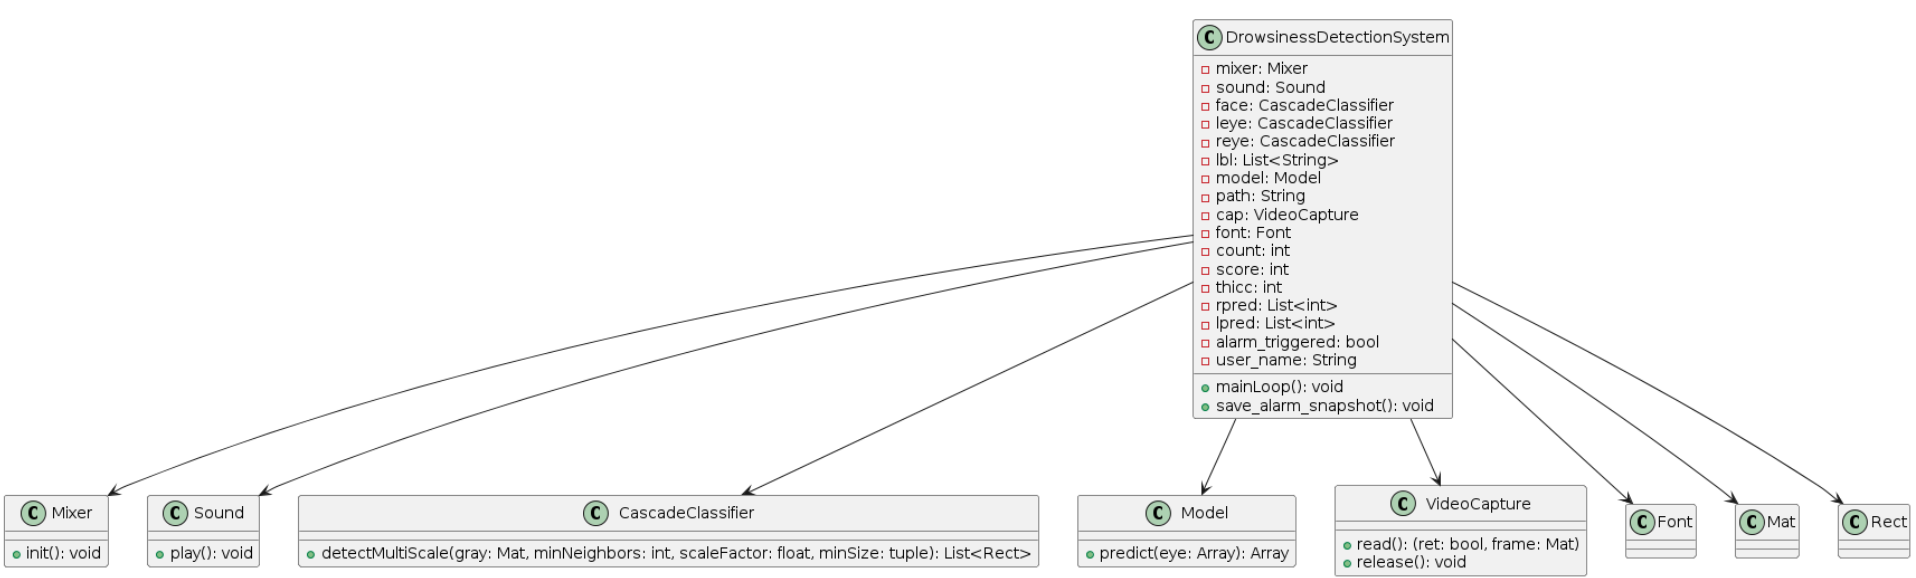
\includegraphics[width=1.0\textwidth]{classdia}
\caption{ Class Diagram}
\end{figure}
\FloatBarrier
 By visually representing the relationships and dependencies among these classes, a class diagram provides a roadmap for developers to implement and maintain the project effectively.


\subsubsection{Sequence Diagram}
A Sequence Diagram illustrates the flow of messages or interactions between objects or components within a system over time. In the context of the provided project, a drowsiness detection system using computer vision, a Sequence Diagram can depict the sequential interactions between various components involved in the process. 

At the core of the system lies the video capturing and processing loop, continuously capturing frames from the webcam. Once a frame is captured, it undergoes a series of steps: face detection, eye detection, preprocessing, and prediction. \\These steps are illustrated as sequential messages exchanged between the main components: the webcam, the face and eye cascade classifiers, the neural network model for eye state prediction, and the alarm system.

When a frame is captured, it undergoes face detection followed by separate detections for left and right eyes. Each detected eye region is then preprocessed and fed into the pre-trained convolutional neural network (CNN) model to predict whether the eye is open or closed. \\Based on these predictions, the system keeps track of the user's drowsiness level by maintaining a score. If the score exceeds a predefined threshold, indicating drowsiness, an alarm is triggered, and a snapshot of the user is saved for logging purposes.

Additionally, interactions with external components are also depicted. For example, when drowsiness is detected, a notification is sent to a Flask server running locally, and in parallel, the alarm sound is played. Furthermore, the system attempts to save the user's name when drowsiness is detected by sending a POST request to the Flask server.

Throughout this process, the Sequence Diagram highlights the sequential flow of operations, interactions, and dependencies between different components of the drowsiness detection system, providing a clear visualization of how the system functions in real-time.
\begin{figure}[h]
\centering
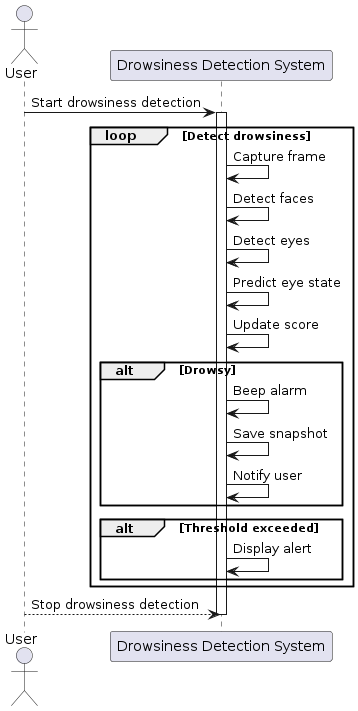
\includegraphics[width=0.4\textwidth]{seq}
\caption{Sequence Diagram}
\end{figure}
\FloatBarrier


\subsubsection{Activity Diagram}

The Drowsiness Detection System is designed to detect driver drowsiness and prevent potential accidents. It operates by analyzing the driver's eye state using a camera. The system utilizes a convolutional neural network (CNN) model to predict whether the driver's eyes are open or closed. Upon detecting drowsiness, an alarm is triggered to alert the driver. 

Additionally, the system captures an image of the drowsy driver for record-keeping. The system is implemented using Python and OpenCV for real-time video processing, and it incorporates Haar cascades for face and eye detection. Below is the activity diagram representing the workflow of the Drowsiness Detection System.
\begin{figure}[h]
\caption{Activity Diagram }
\centering
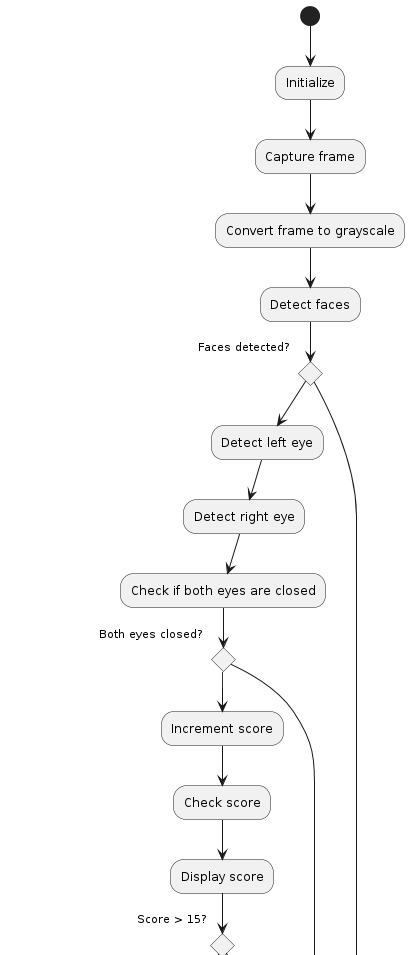
\includegraphics[width=0.6\textwidth]{act1}
\end{figure}
\FloatBarrier
\begin{figure}[h]
\centering
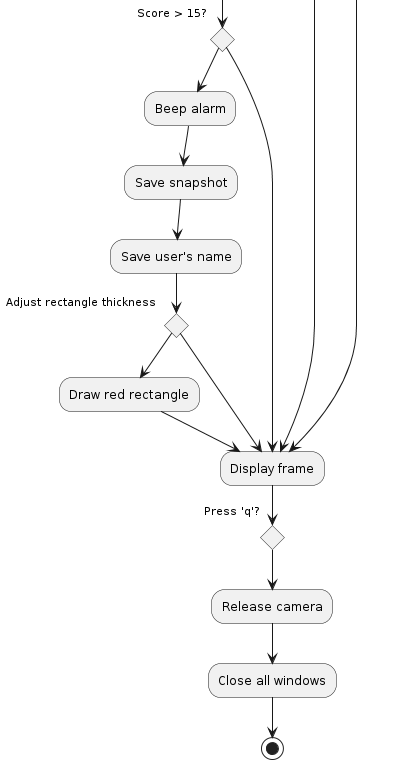
\includegraphics[width=0.7\textwidth]{act2}
\end{figure}
\FloatBarrier


\subsubsection{Use Case}
The Drowsiness Detection System represents a crucial innovation in the realm of road safety, leveraging advanced technologies to address the persistent issue of accidents caused by drowsy driving. With its foundation built upon computer vision and machine learning, the system stands as a proactive guardian against potential disasters on the road. Its multifaceted approach begins with the intricate task of facial landmark detection. By meticulously tracking key facial features, including the eyes and head, the system establishes a baseline for monitoring the driver's alertness.

Central to the system's efficacy is its continuous monitoring of eye closure patterns. Through sophisticated algorithms, the system analyzes subtle changes in eye behavior, promptly identifying instances of prolonged eye closure indicative of drowsiness or fatigue. This real-time assessment serves as an early warning system, allowing for timely intervention to prevent potential accidents. Concurrently, the system tracks head movements, recognizing sudden or erratic shifts that may signal a lapse in concentration. By integrating these insights, the system paints a comprehensive picture of the driver's state, enabling proactive measures to maintain road safety.
\begin{figure}[h]
\centering
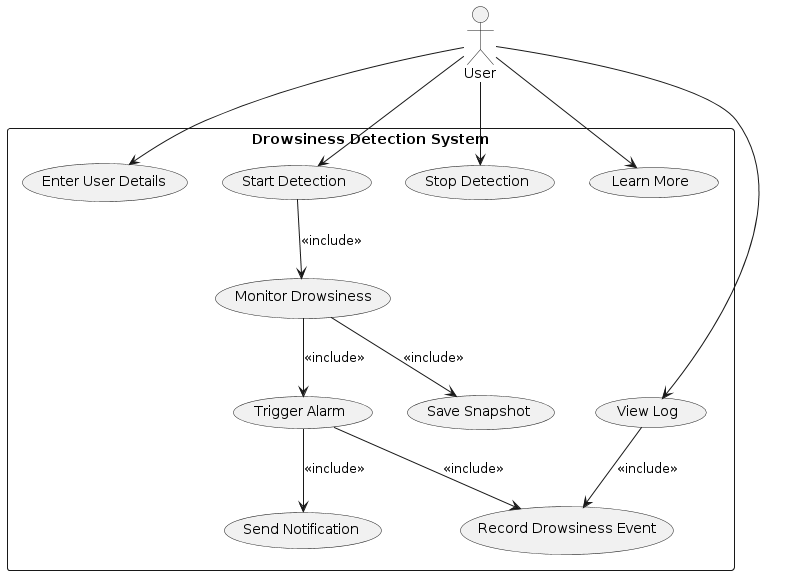
\includegraphics[width=1.0\textwidth]{use}
\caption{Use Case Diagram}
\end{figure}
\FloatBarrier

The cornerstone of the Drowsiness Detection System lies in its ability to detect and respond to signs of drowsiness promptly. Upon recognizing concerning patterns in eye closure or head movements, the system initiates a series of actions aimed at alerting the driver and mitigating the risk of accidents. An alarm, carefully calibrated to garner attention without causing undue distraction, serves as the primary means of notification. Whether through auditory cues, visual alerts, or tactile feedback, the alarm effectively jolts the driver out of complacency, prompting them to reorient their focus and take necessary precautions.

In addition to its real-time intervention capabilities, the system incorporates features designed to support post-event analysis and accountability. A comprehensive logging mechanism records pertinent details, including the time of detection, driver information, and system response. This data not only facilitates performance evaluation and system refinement but also serves as a valuable resource for accident investigations and regulatory compliance.

Beyond its technical intricacies, the Drowsiness Detection System embodies a broader commitment to road safety and societal well-being. By proactively addressing the root causes of drowsy driving, the system contributes to a culture of responsibility and awareness on the road. Moreover, its potential for integration into various vehicular platforms opens avenues for widespread adoption, extending its impact across diverse demographics and geographical regions.

\subsubsection{Use Case Purpose}

The Drowsiness Detection System is designed to detect driver drowsiness and prevent potential accidents. The system uses a webcam to monitor the driver's face in real-time. It employs Haar cascades for face and eye detection and a Convolutional Neural Network (CNN) model for eye state prediction. When the driver's eyes are closed for an extended period, indicating drowsiness, the system triggers an alarm to alert the driver. Additionally, it captures an image of the drowsy driver for future reference. This system aims to enhance road safety by preventing accidents caused by driver fatigue.\\

- Indian Government Report Reference: According to a report by the Ministry of Road Transport and Highways, Government of India, driver fatigue is one of the leading causes of road accidents in the country. Implementing systems like Drowsiness Detection can significantly reduce such accidents, thereby saving lives and minimizing economic losses.

\subsubsection{COMPONENT DIAGRAM }
A component diagram for the Drowsiness Detection System can illustrate the modular structure and interactions within the system's various components. In this context, the system comprises several interconnected components: 

At its core, the system involves three main components : the Python-based drowsiness detection algorithm, the web server, and the user interface. 

The Python code encompasses the drowsiness detection algorithm, leveraging computer vision libraries like OpenCV and machine learning models for eye state prediction. It orchestrates tasks such as capturing video frames, processing facial landmarks, and triggering alarms when drowsiness is detected. 

The web server serves as the intermediary between the Python code and the user interface, facilitating communication and data exchange. It handles HTTP requests and responses, enabling functionalities like setting user details, starting and stopping drowsiness detection, and logging detection events.

The user interface, developed using HTML, CSS, and JavaScript, presents an interactive platform for users to engage with the system. It includes components such as the main page for user input, a learn more page for system insights, and a log page for recording detection events.
\begin{figure}[h]
\centering
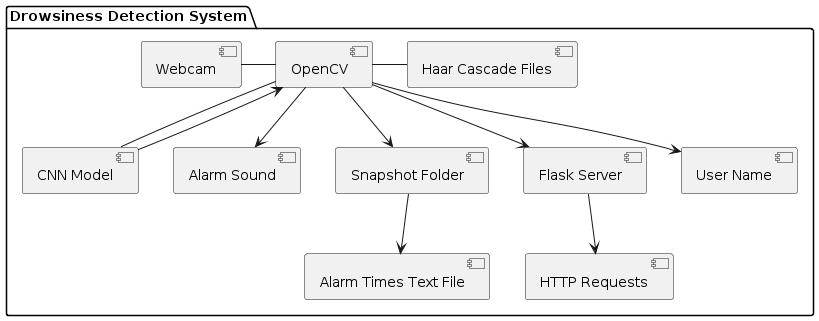
\includegraphics[width=1.0\textwidth]{CD}
\caption{Component Diagram}
\end{figure}
\FloatBarrier
Moreover, the system integrates additional components such as audio and visual alerts, data logging, and user authentication to enhance its functionality and usability. For instance, audio alerts notify users of drowsiness, while visual alerts highlight drowsiness events on the user interface. Data logging records user details and detection timestamps for future reference. 


By visually mapping these components and their interactions, the component diagram provides a comprehensive overview of the Drowsiness Detection System's architecture, aiding in system understanding, development, and maintenance.


\subsubsection{DEPLOYMENT DIAGRAM }
A deployment diagram illustrates the physical deployment of software components within a system. In the context of the Drowsiness Detection System, the deployment diagram outlines the distribution of software elements across various nodes or hardware devices.

The system comprises several components, including a Python script for drowsiness detection utilizing OpenCV, Keras, and Pygame libraries (code 1), a Flask web application (code 2), HTML page for learning more about the system (code 3), a log display page (code 4), and the main user interface for drowsiness detection (code 5).

The deployment of these components involves running the Python script on a device equipped with a camera for real-time monitoring of the user's facial landmarks. The Flask web application serves as the interface for user interaction, providing a form for user details and displaying system guidelines. The HTML pages for learning more and viewing logs are served by the Flask app. Additionally, the main user interface, which incorporates the drowsiness detection functionality, is presented through an HTML page that communicates with the Python script running in the background.

The deployment diagram depicts these components deployed across different nodes, with the Python script executing on a local machine, and the Flask app hosted on a server accessible via localhost. The user interacts with the system through a web browser, enabling seamless integration and user-friendly access to the drowsiness detection functionality.


\begin{figure}[h]
\centering
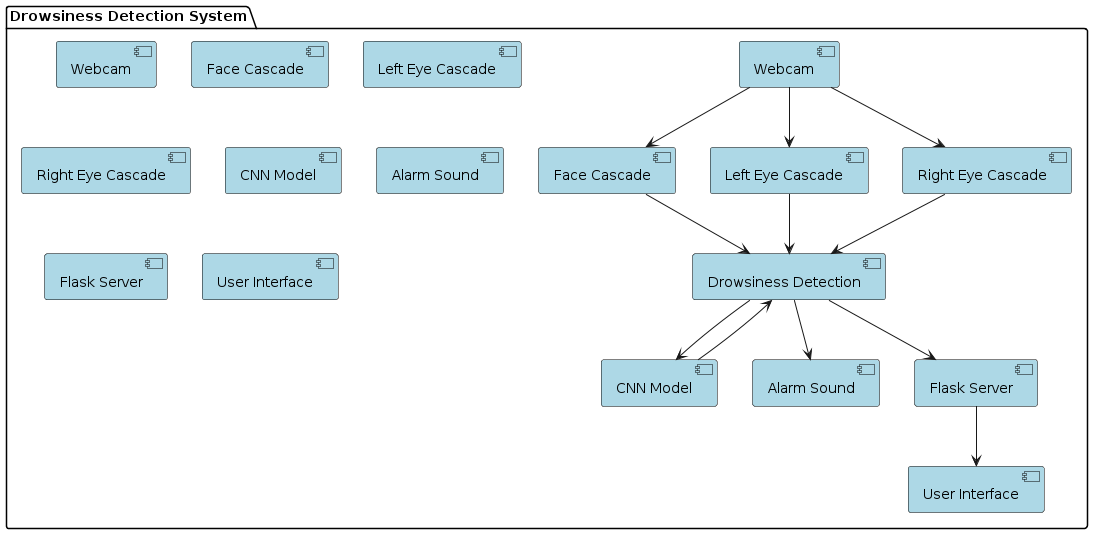
\includegraphics[width=1.0\textwidth]{DeD}
\caption{Deployment Diagram }
\end{figure}
\FloatBarrier
The system utilizes the following components:\\
- Webcam: The system captures video input from the webcam to monitor the driver's face.\\
- Haar Cascades: These are pre-trained classifiers used for face and eye detection. The system uses Haar cascades to identify faces and eyes in the video stream.\\
- Convolutional Neural Network (CNN) Model: This model is responsible for predicting the state of the driver's eyes (open or closed). The CNN model is trained to detect eye states using pre-labeled eye images.\\
- Alarm Sound: An alarm sound is played when the system detects drowsiness in the driver. 

Furthermore, the deployment diagram highlights the integration of the drowsiness detection system into everyday scenarios, such as in vehicles or workspaces, where fatigue-related accidents pose significant risks. By deploying the system across appropriate hardware devices, such as embedded systems within vehicles or dedicated monitoring stations, the detection of drowsiness becomes proactive, contributing to enhanced safety measures. This strategic deployment ensures that the system can be easily accessed and utilized by individuals requiring continuous monitoring of their alertness levels, thereby mitigating the potential dangers associated with drowsy driving or operating machinery. 

\newpage
\section{PROJECT PLAN }
\textbf{1. Project Overview:}

   - The Drowsiness Detection System aims to prevent accidents caused by driver fatigue by continuously monitoring the driver's alertness level.

   - The system utilizes computer vision techniques to track facial landmarks, eye closure, and head movements in real-time.

   - When drowsiness is detected, the system triggers an alarm to alert the driver, thereby preventing potential accidents.\\
\textbf{2. Project Components:}

   - Software Development: Develop software components for facial landmark detection, eye closure monitoring, head movement tracking, and alarm triggering.
   
   - Integration: Integrate individual components to create a cohesive system for drowsiness detection.

   - User Interface: Develop user interfaces for system interaction, including a web application for user registration and monitoring.

   - Testing: Perform thorough testing to ensure the reliability and accuracy of the detection system under various conditions.

   - Deployment: Deploy the system for real-world usage, potentially integrating it into vehicles or other relevant environments.\\
\textbf{3. Software Development Tasks:}

   - Facial Landmark Detection: Implement algorithms for detecting and tracking facial landmarks using computer vision libraries such as OpenCV.

   - Eye Closure Monitoring: Develop algorithms to monitor eye closure by analyzing changes in eye behavior captured by the camera.

   - Head Movement Tracking: Implement techniques to track head movements and assess the driver's alertness level based on the detected movements.

   - Alarm Triggering: Develop mechanisms to trigger an alarm when drowsiness is detected, including sound, visual, or haptic alerts.

   - User Interface Development: Create user interfaces for system interaction, including a web-based interface for user registration and monitoring.\\
\textbf{4. Integration and Testing:}

   - Integration: Integrate the individual software components into a unified system for drowsiness detection.

   - Functional Testing: Conduct functional testing to ensure that each component performs its intended function accurately.

   - Performance Testing: Assess the system's performance under various conditions, including different lighting conditions and driver behaviors.

   - User Acceptance Testing: Involve end-users in testing to gather feedback and make improvements based on user experience.\\
\textbf{5. Deployment and Monitoring:}

   - Deployment Strategy: Determine the deployment strategy, considering factors such as hardware requirements, scalability, and maintenance.

   - Monitoring and Maintenance: Establish monitoring mechanisms to track the system's performance in real-world usage and address any issues promptly.

   - User Training: Provide training to end-users on how to interact with the system effectively and respond to alerts appropriately.\\
\textbf{6. Documentation and Reporting:}

   - Documentation: Prepare comprehensive documentation covering system architecture, installation instructions, user guides, and troubleshooting procedures.

   - Project Report: Compile a detailed project report summarizing the development process, challenges faced, solutions implemented, and outcomes achieved.\\
\textbf{7. Timeline:}

   - Phase 1 (Development): [Specify Start and End Dates]

   - Phase 2 (Testing): [Specify Start and End Dates]

   - Phase 3 (Deployment): [Specify Start and End Dates]\\
\textbf{8. Resources and Responsibilities:}

   - Development Team: [List Team Members and Their Roles]

   - Testing Team: [List Team Members and Their Roles]

   - Project Manager: [Name and Responsibilities]\\
\textbf{9. Risk Management:}

   - Identify potential risks such as technical challenges, resource constraints, and regulatory compliance issues.

   - Develop mitigation strategies to address identified risks and minimize their impact on project timelines and outcomes.\\
\textbf{10. Conclusion:}

    - The successful implementation of the Drowsiness Detection System will contribute to enhancing road safety and preventing accidents caused by driver fatigue.

\subsection{ PROJECT ESTIMATE }
The project entails the development of a sophisticated Drowsiness Detection System leveraging a combination of computer vision and machine learning methodologies to mitigate the risks associated with driver fatigue-induced accidents. It initiates with an in-depth Research and Planning phase, allocating approximately 1 week for reviewing existing systems, defining project requirements, and outlining the project scope. 

Subsequently, the Data Collection and Preparation phase, estimated at 2 weeks, involves gathering a diverse dataset of images and videos capturing various instances of drowsiness, necessitating meticulous labeling and preprocessing for subsequent model training. The Model Development phase, slated for 4 weeks, encompasses the creation and refinement of a robust deep learning model capable of accurately detecting signs of drowsiness by analyzing facial landmarks and eye movements. Integration and Testing follow, requiring 3 weeks for seamlessly incorporating the model into the system framework, conducting rigorous testing, debugging, and optimizing performance for real-world scenarios. 

Concurrently, User Interface Development, spanning 2 weeks, focuses on designing and implementing intuitive interfaces, particularly web-based platforms, facilitating user interaction and data visualization. Documentation and Reporting, slated for 2 weeks, entail the comprehensive documentation of system architecture, implementation details, user guidelines, and technical specifications, culminating in the preparation of a detailed project report. The estimated 9-week timeline is subject to adjustments based on factors such as resource availability, unforeseen technical challenges, and evolving project requirements. Post-deployment, ongoing Deployment and Maintenance activities involve continual system monitoring, optimization, and user support to ensure long-term effectiveness and reliability.

\begin{figure}[h]
\centering
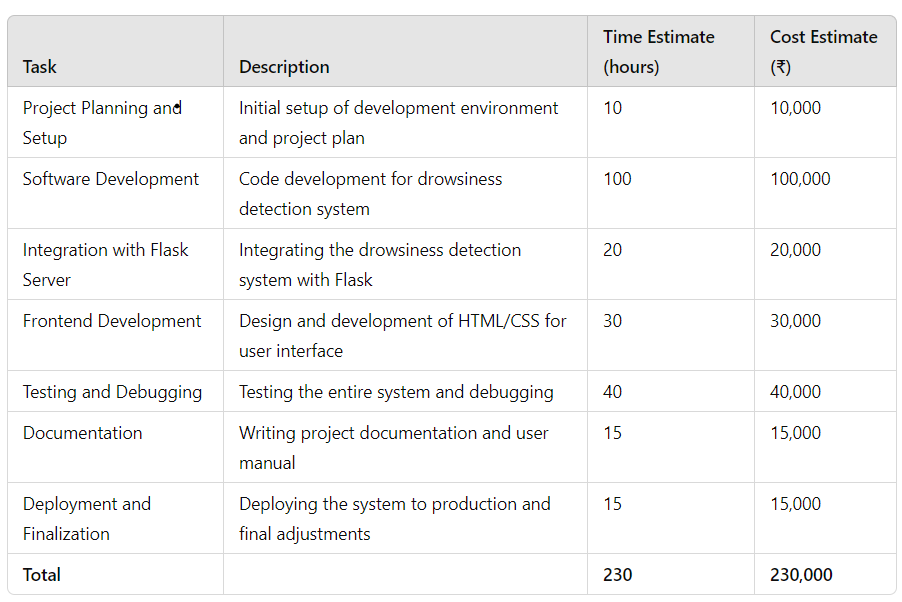
\includegraphics[width=1.0\textwidth]{estimate}
\caption{Estimate }
\end{figure}
\FloatBarrier


\subsection{RISK MANAGEMENT }
Risk management is a crucial aspect of any project, including the Drowsiness Detection System outlined in the provided code. Several risks are associated with the development and deployment of this system, which need to be addressed to ensure its successful implementation and operation.

Firstly, there is a risk related to the accuracy and reliability of the drowsiness detection algorithm. Since the system relies on computer vision techniques to monitor facial landmarks, track eye closure, and detect head movements, any inaccuracies in these processes could lead to false positives or false negatives in drowsiness detection. To mitigate this risk, extensive testing and validation of the algorithm against various scenarios and conditions are necessary.

Secondly, there is a risk of technical failures, such as hardware malfunctions or software bugs, which could affect the system's performance. For instance, if the camera or sensors used for facial recognition and eye tracking malfunction, the system may fail to detect drowsiness accurately. To address this risk, thorough testing of the hardware components and robust error handling mechanisms in the software are essential.

Additionally, there is a risk associated with user acceptance and compliance. Users may be resistant to using the drowsiness detection system, or they may not follow the recommended procedures for its use, such as providing accurate personal information or adhering to safety guidelines while driving. Educating users about the importance of the system and providing clear instructions for its use can help mitigate this risk.

Furthermore, there are legal and ethical risks, particularly concerning privacy and data protection. Since the system collects and processes personal data, there is a risk of violating privacy laws or exposing sensitive information to unauthorized parties. Implementing strict data security measures, obtaining necessary consent from users, and complying with relevant regulations can help mitigate these risks.

\begin{figure}[h]
\centering
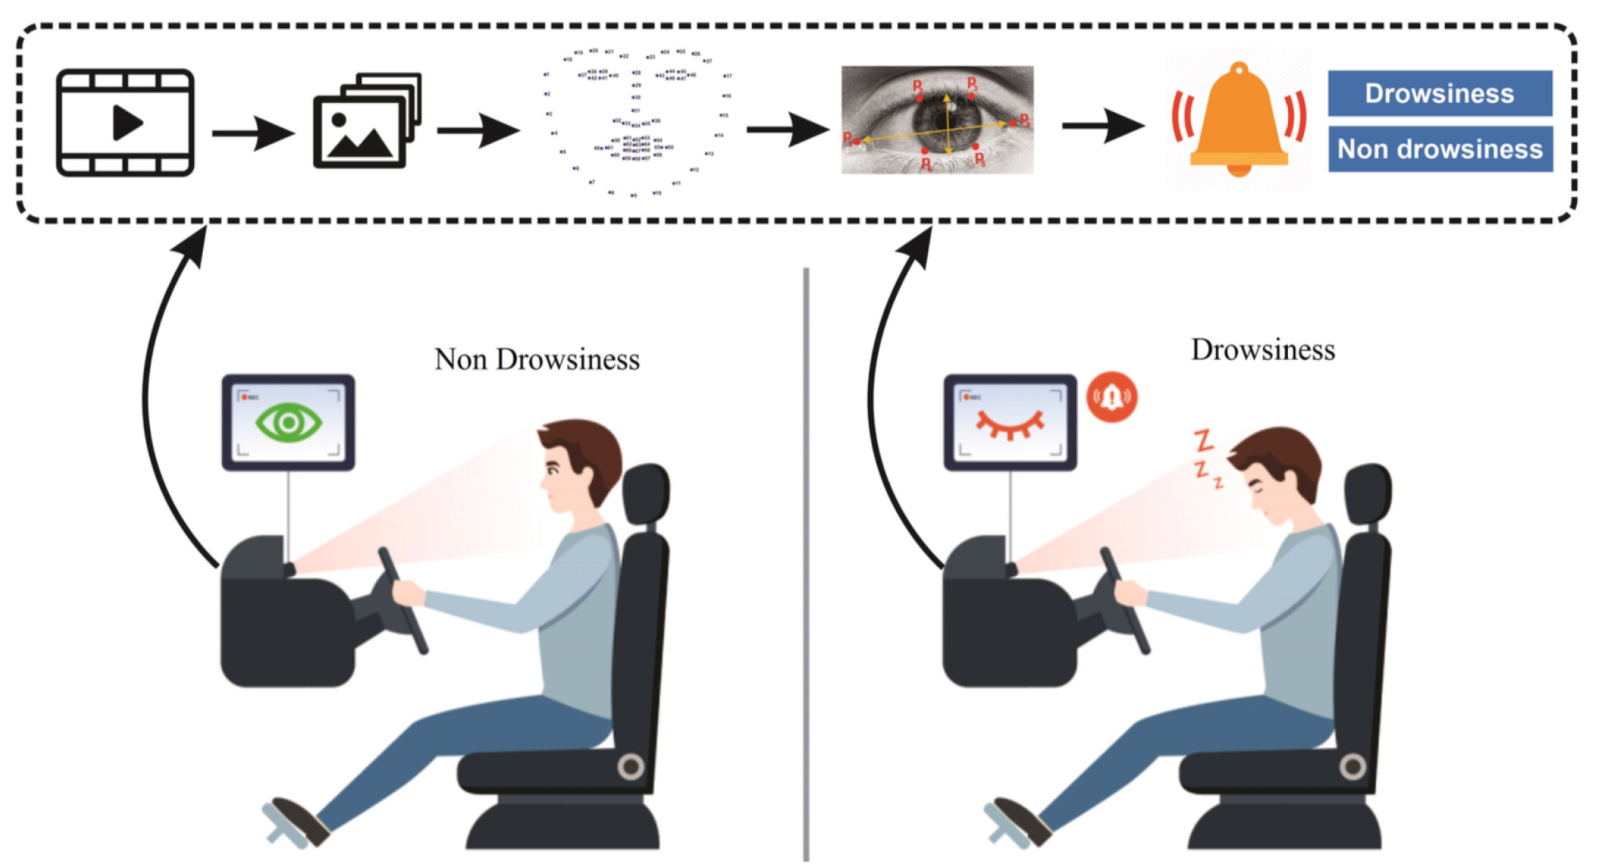
\includegraphics[width=0.8\textwidth]{risk}
\caption{Risk Alert}
\end{figure}
\FloatBarrier

Overall, effective risk management strategies, including thorough testing, robust technical solutions, user education, and compliance with legal and ethical standards, are essential to ensure the success and safety of the Drowsiness Detection System.

\subsubsection{Types Of Risk}

\begin{itemize}
\item Technical Risk\\
   - Risk Description:\\
     - Drowsiness detection system may fail due to technical issues such as poor lighting conditions or occlusion of the driver's face.\\
   - Probability: Medium\\
   - Impact: High\\
   
\item Operational Risk\\
   - Risk Description:\\ 
     - Inaccurate drowsiness detection due to improper positioning of the driver in front of the camera.\\
   - Probability: Medium\\
   - Impact: High\\
   
\item System Risk\\
   - Risk Description:\\ 
     - Drowsiness detection system may malfunction, leading to failure in alerting the driver of drowsiness.\\
   - Probability: Medium\\
   - Impact: High\\
\end{itemize}
\subsubsection{Risk Probability }
The risk probability table outlines potential challenges faced during the development and implementation of the drowsiness detection system. Environmental factors may hinder face detection accuracy, posing a high risk due to its impact on system functionality. Additionally, inaccuracies in predicting eye states could lead to false alarms, increasing the risk level. Hardware failures and insufficient computational resources pose medium risks, affecting system reliability. Adequate training data and user awareness mitigate risks, while integration issues and performance degradation present moderate concerns. Proactive risk management ensures smoother project execution and enhances system effectiveness, safeguarding against potential disruptions.

\begin{figure}[h]
\centering
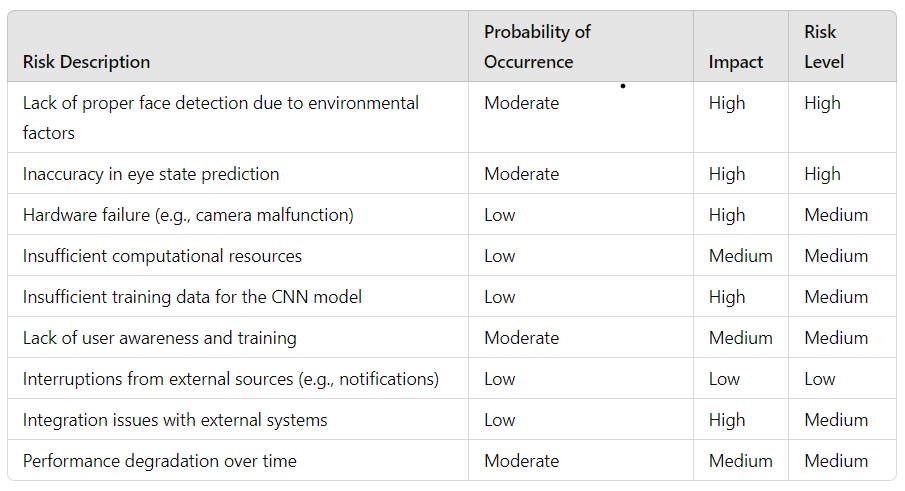
\includegraphics[width=1.0\textwidth]{probab}
\caption{Risk Probability}
\end{figure}
\FloatBarrier

\subsubsection{Risk Impact }
Risk impact refers to the severity of the consequences that may arise if a risk event occurs during the development and deployment of the drowsiness detection system. In this context, the impact encompasses various dimensions, including technical, operational, financial, and reputational aspects. 

From a technical standpoint, risks such as inaccuracies in eye state prediction or hardware failures can directly compromise the system's functionality, potentially leading to false alarms or, worse, failing to detect drowsiness in critical situations. These technical challenges can undermine the system's reliability and effectiveness, ultimately endangering road safety.

Operationally, risks like integration issues with external systems or insufficient computational resources can disrupt the smooth operation of the drowsiness detection system. Integration issues may lead to delays or inconsistencies in data processing, while inadequate computational resources may hinder real-time monitoring capabilities, reducing the system's responsiveness.

Financially, the impact of risks can manifest in increased project costs due to the need for additional resources to address technical challenges or mitigate system failures. Moreover, reputational damage may occur if the system fails to meet expectations or experiences frequent disruptions, eroding trust among users and stakeholders.

Overall, understanding and mitigating the potential impact of risks are crucial for ensuring the successful development, deployment, and long-term sustainability of the drowsiness detection system. Effective risk management strategies are essential to minimize negative consequences and maximize the system's ability to fulfill its intended purpose of preventing accidents and saving lives on the road.
\subsubsection{Risk Description}
The risk description table presents a holistic view of potential challenges that may impact the development and deployment of the drowsiness detection system. High probabilities of occurrence, coupled with significant impacts, highlight critical areas such as regulatory compliance, data privacy breaches, and resource constraints. 

\begin{figure}[h]
\centering
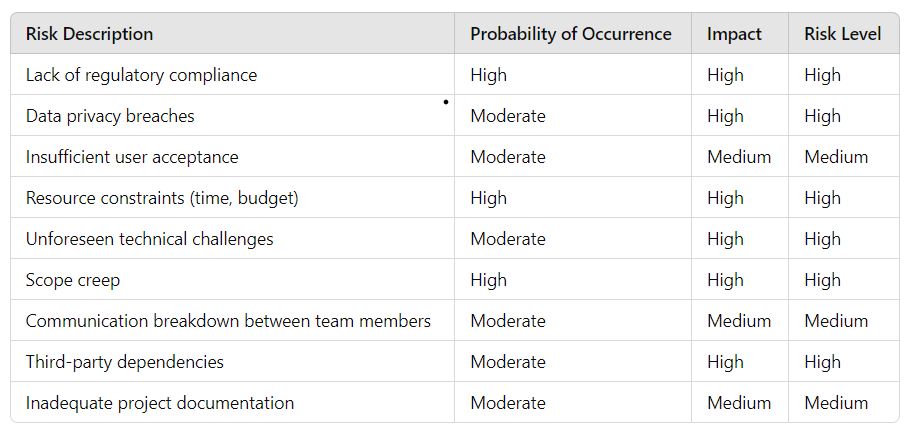
\includegraphics[width=1.0\textwidth]{des}
\caption{Risk Description}
\end{figure}
\FloatBarrier

These risks pose considerable threats to project success and road safety, demanding proactive mitigation strategies. Moderate risks, such as technical challenges and communication breakdowns, also warrant attention to prevent disruptions in system development and ensure effective collaboration among team members. Prioritizing risk management efforts based on probability, impact, and risk level is essential for navigating complexities and achieving project objectives.
\newpage

\section{PROJECT IMPLEMENTATION}
The project implementation involves the development of a Drowsiness Detection System using computer vision techniques and machine learning models. The system is designed to prevent accidents caused by driver fatigue by continuously monitoring the driver's alertness level and triggering an alarm when drowsiness is detected.\\
The implementation consists of several components:\\

\textbf{1. Python Implementation :}

- The core functionality of the system is implemented in Python using OpenCV for face and eye detection, Keras for eye state prediction, and Pygame for audio alerts. 

- The system captures video frames from a webcam, detects faces and eyes, analyzes eye closure patterns, and triggers an alarm if drowsiness is detected.

- Additionally, it saves snapshots when the alarm is triggered for further analysis.

\textbf{2. Web Interface :}

- The system includes a web-based user interface developed using HTML, CSS, and JavaScript. Users can input their details such as name, age, and gender through a form.

- Upon submission, the system starts monitoring the user's alertness level.

- The interface also provides a "Learn More" section to educate users about the system's functionality.

- Additionally, users can view their details and log records to track their drowsiness incidents.

Overall, the implementation seamlessly integrates real-time video processing, machine learning algorithms, and user interaction to create an effective Drowsiness Detection System aimed at enhancing road safety.

\subsection{OVERVIEW OF PROJECT MODULES }
This project aims to develop a drowsiness detection system using a webcam to monitor the driver's eyes in real-time. The system consists of the following modules:\\
\begin{itemize}
\item Image Acquisition: Captures the driver's image using a webcam.
   
\item Face and Eye Detection: Uses Haar cascades to detect faces and eyes in the images.
   
\item Eye State Prediction: Utilizes a Convolutional Neural Network (CNN) to predict the state of the driver's eyes (open/closed).
   
\item Drowsiness Detection: Monitors the driver's eyes continuously. If closed beyond a threshold, an alarm is triggered to alert the driver.
   
\item Alert System: Plays an alarm sound to alert the drowsy driver.
   
\item Snapshot Capture: Takes an image of the drowsy driver for record-keeping and analysis.
\end{itemize}
\subsection{OVERVIEW OF ADMIN AND USER MODULE}
The Drowsiness Detection System comprises two essential modules: the Admin Module and the User Module, each serving distinct purposes in ensuring the functionality and effectiveness of the system.
\subsubsection{Admin Module:}

The Admin Module serves as the backbone of the Drowsiness Detection System, facilitating the management and configuration of the system parameters. Admin functionalities include:\\

\textbf{- Model and Cascade Loading: }

The module initializes the necessary components such as Haar cascades for face and eye detection and the Convolutional Neural Network (CNN) model for eye state prediction.\\

\textbf{- Alarm Sound Setup: }

It configures the alarm sound that triggers upon detecting drowsiness, employing pygame mixer for sound management.\\

\textbf{- Snapshot and Logging:} 

Admin functionalities extend to saving snapshots upon drowsiness detection, along with logging timestamped data for further analysis.\\

\textbf{- User Interaction: }

The module interacts with the User Module, receiving user details and forwarding alarm triggers to the user interface for real-time alerts.\\

\subsubsection{User Module:}
The User Module serves as the interface through which users interact with the Drowsiness Detection System. Key features of the User Module include:\\

\textbf{- User Registration: }

Users provide their details such as name, age, and gender through a web form to personalize the system's alerts and records.\\

\textbf{- Alert Display:} 

Upon registration, users receive personalized alerts regarding their drowsiness status during real-time monitoring.\\

\textbf{- System Interaction:} 

Users can start and stop the drowsiness detection process through intuitive controls, ensuring proactive engagement with the system.
\newpage

\section{ TOOLS AND TECHNOLOGIES USED }

This project employs a variety of tools and technologies to achieve its objectives:\\
\textbf{1. Python (Programming Language):}

Python is used extensively for backend development and machine learning model training. Its simplicity and vast array of libraries make it ideal for implementing complex algorithms, handling data processing, and developing web applications. In this project, Python's versatility allows for seamless integration of various components, from computer vision to web frameworks.\\
\textbf{2. OpenCV (Open Source Computer Vision Library):}

OpenCV is leveraged for real-time computer vision tasks such as face detection, eye detection, and image processing. It provides a comprehensive set of tools to perform operations on images and videos, enabling the system to detect facial features and monitor eye states effectively. The use of OpenCV ensures accurate and efficient image analysis.\\
\textbf{3. NumPy (Numerical Python):}

NumPy is employed for efficient numerical computations and data manipulation. It is particularly useful in preprocessing image data, where it handles large arrays and matrices. NumPy's powerful capabilities make it indispensable for tasks that require mathematical operations on pixel values during the image processing phase.\\
\textbf{4. Keras (Deep Learning Library):}

Keras is used for building and training the Convolutional Neural Network (CNN) model for eye state prediction. Its user-friendly API facilitates the creation and deployment of deep learning models. In this project, Keras helps in designing a model that can accurately distinguish between open and closed eye states, crucial for drowsiness detection.\\
\textbf{5. pygame (Python Library for Multimedia Applications):}

pygame is integrated for playing the alarm sound when drowsiness is detected. This library handles audio playback, allowing the system to alert the user with a sound when necessary. Its ease of use and flexibility make it a suitable choice for multimedia tasks within Python applications.\\
\textbf{6. Requests (Python HTTP Library):}

Requests is incorporated for making HTTP requests to communicate with the Flask server. It simplifies the process of sending HTTP requests, enabling the system to interact with the backend efficiently. This communication is essential for tasks like notifying the server when an alarm is triggered or sending user data.\\
\textbf{7. Flask (Python Web Framework):}

Flask is utilized to develop the web application backend for user interaction and data handling. It provides a lightweight and flexible framework for building web applications, making it easier to manage routes, handle user input, and serve dynamic content. Flask's simplicity and scalability are key for developing the project's web components.\\
\textbf{8. HTML (Hypertext Markup Language):}

HTML is employed for creating the structure and content of the web pages in the frontend. It defines the layout and elements of the user interface, ensuring a well-organized presentation of information. HTML forms the backbone of the web application's visual framework.\\
\textbf{9. CSS (Cascading Style Sheets):}

CSS is utilized for styling the HTML elements and enhancing the visual appearance of the web pages. It provides the ability to apply styles, such as colors, fonts, and layouts, ensuring that the web application is both attractive and user-friendly. CSS is crucial for creating a cohesive and appealing design.\\
\textbf{10. JavaScript:}

JavaScript is used for client-side scripting to handle user interactions and dynamic content updates. It enables the web application to be interactive, responding to user actions such as form submissions and button clicks. JavaScript enhances the overall user experience by making the web pages more responsive and functional.\\
\textbf{11. Haar Cascades:}

Haar Cascades are XML files utilized for face and eye detection using Haar feature-based cascade classifiers. These pre-trained classifiers enable the system to detect facial features quickly and accurately. Haar Cascades are essential for identifying regions of interest in images for further processing by the CNN model.\\
\textbf{12. Operating System APIs (e.g., `os` module):}

Operating System APIs, such as Python's `os` module, are utilized for file operations, such as accessing directories, managing paths, and saving snapshots. These functions allow the system to handle file storage and retrieval tasks efficiently, ensuring that data is organized and accessible for analysis and logging.\\


\subsection{HARDWARE RESOURCES REQUIRED }

\textbf{1. Camera :}

- A camera is required to capture the video feed of the driver's face. This can be a webcam integrated into the device or an external camera connected to the system.\\

\textbf{2. Speakers or Headphones :} 

- Audio output devices are needed to produce alarm sounds when drowsiness is detected. This can include built-in speakers or external speakers connected to the system, or headphones plugged into the audio jack.\\

\textbf{3. Computer or Embedded System :}

- The system requires a computing device capable of running the Python script and hosting the Flask web server. This can range from a desktop or laptop computer to a dedicated embedded system with sufficient processing power and memory.\\

\textbf{4. Internet Connection (Optional) :} 

An internet connection may be necessary if the system is designed to interact with external services, such as sending notifications or accessing online resources.\\

\textbf{5. Storage :}

- Sufficient storage space is required to store the Python script, Haar cascade files for face and eye detection, CNN model for eye state prediction, alarm sound file, and any captured images or log files generated during runtime.\\

\textbf{6. Additional Components (Optional) :}

- Depending on the specific implementation, additional components such as microphones for audio input, LED indicators for visual alerts, and power supply units may be required.\\

\textbf{7. Operating System :} 

-The system can run on various operating systems such as Windows, Linux, or macOS, depending on the compatibility of the required software libraries and drivers.
This system does not require any specialized hardware components beyond a standard computer setup.\\

\subsection{SOFTWARE RESOURCES REQUIRED}
"SOFTWARE RESOURCES REQUIRED:

\textbf{1. Python : }

- The project is developed using Python programming language, which is essential for running the provided code.\\

\textbf{2. OpenCV : }

- OpenCV (Open Source Computer Vision Library) is utilized for image and video processing tasks, particularly for face and eye detection.\\

\textbf{3. NumPy : }

- NumPy is employed for numerical computing and array manipulation, which is crucial for processing images and data arrays efficiently.\\

\textbf{4. Keras : }

- Keras, a high-level neural networks API, is necessary for loading and utilizing the pre-trained deep learning model for eye state prediction.\\

\textbf{5. pygame : }

- Pygame is used for playing sound alarms in the application when drowsiness is detected.\\

\textbf{6. Requests : }

- The Requests library is used for making HTTP requests, particularly for sending alerts to a Flask server when drowsiness is detected and to set user details.\\

\textbf{7. Flask (not included) :}

- While not explicitly included in the provided code, a Flask server is assumed to be running locally on the system to handle HTTP requests for setting user details, triggering alarms, and logging records.\\

\textbf{8. Haar Cascade Files : }

- Haar cascade XML files for face and eye detection are required, which are provided in the 'haar cascade files' directory.\\

\textbf{9. Pre-trained CNN Mode l:} 

- A pre-trained Convolutional Neural Network (CNN) model for eye state prediction (cnncat2.h5) is necessary for determining whether the eyes are open or closed.\\

\textbf{10. Sound File : }

- An alarm sound file (alarm.wav) is essential for auditory alerts when drowsiness is detected.\\

\textbf{11. Static Files for Web Interface (HTML, CSS, JS) :} 

- HTML, CSS, and JavaScript files are utilized for creating the web interface of the Drowsiness Detection System, along with static images for backgrounds and icons.\\

\textbf{Note :} "Ensure all necessary dependencies and files are present and properly configured for the smooth execution of the project."

\subsubsection{Why Python?}
In the context of the provided project, Python is used due to several reasons:

\textbf{1. Libraries and Frameworks : }

- Python offers extensive libraries and frameworks suitable for computer vision tasks and web development. In this project, libraries such as OpenCV, Keras, and Flask are utilized for image processing, machine learning model implementation, and web server development, respectively.\\

\textbf{2. Ease of Development :}

- Python's syntax is concise and easy to understand, making it ideal for rapid development. This is crucial for projects with tight deadlines or where quick iterations are necessary, as in the case of this drowsiness detection system.\\

\textbf{3. Community Support :}

- Python has a large and active community of developers, which means there are abundant resources, tutorials, and forums available for troubleshooting and assistance. This can be particularly helpful when encountering issues or seeking optimizations in the project.\\

\textbf{4. Integration : }

- Python seamlessly integrates with other languages and technologies. In this project, Python is used for both backend (drowsiness detection algorithm) and frontend (web interface), ensuring smooth communication between the different components of the system.\\

\textbf{5. Platform Independence : }

- Python is platform-independent, meaning the code can run on various operating systems without modification. This flexibility is advantageous for deployment on different devices or environments.\\

\textbf{6. Scalability : }

- Python's scalability allows for easy scaling of the project as requirements evolve. Whether it's adding new features, handling increased user load, or deploying on different hardware configurations, Python offers scalability options.\\

Overall, Python's versatility, ease of use, and robust ecosystem make it a suitable choice for developing the drowsiness detection system, encompassing both the backend algorithm for real-time monitoring and the frontend web interface for user interaction.

\subsection{LIBRARIES USED }
\begin{itemize}
\item cv2 (OpenCV):\\
OpenCV is a popular computer vision library used for various image and video processing tasks.\\
In this code, OpenCV is used for:
\begin{itemize}
\item Capturing video frames from the camera (cap = cv2.VideoCapture(0)).
\item Performing face and eye detection using Haar cascades (cv2.CascadeClassifier).
\item Drawing rectangles around detected faces and eyes (cv2.rectangle).
\item Converting frames to grayscale (cv2.cvtColor).
\item Displaying frames (cv2.imshow) and handling window events (cv2.waitKey).
\item Releasing the camera and closing OpenCV windows.
\end{itemize}
\item os:
\begin{itemize}
\item The os module provides functions for interacting with the operating system.
\item It is used here for:
\item Getting the current working directory (os.getcwd()).
\item Creating directories and managing file paths (os.path.join, os.makedirs).
\end{itemize}
\item numpy (np):
\begin{itemize}
\item NumPy is a powerful library for numerical computing in Python.
\item It is used here for handling arrays and numerical operations (np.array, np.expandDims).
\end{itemize}

\item keras.models:
\begin{itemize}
\item Keras is a high-level neural networks API running on top of TensorFlow or Theano.
\item The loadModel function is used here to load a pre-trained CNN model for eye state prediction (loadMdel('models/cnncat2.h5')).
\end{itemize}
\item pygame.mixer:
\begin{itemize}
\item Pygame is a cross-platform set of Python modules designed for writing video games.
\item The pygame.mixer module is used here for:
\item Initializing the mixer (mixer.init()).
\item Loading and playing the alarm sound (mixer.Sound('alarm.wav')).
\end{itemize}

\item datetime:

\begin{itemize}
\item The datetime module supplies classes for manipulating dates and times.
\item It is used here for:
\item Getting the current time (datetime.datetime.now()).
\item Formatting time for file naming (strftime).
\end{itemize} 

\item requests:
\begin{itemize}
\item Requests is an elegant and simple HTTP library for Python.
\item It is used here for:
\item Sending HTTP GET and POST requests to a Flask server (requests.get, requests.post).
\end{itemize}
\end{itemize}
\subsection{ALGORITHM DETAILS }


\textbf{1. Import Libraries:}

- The necessary libraries such as OpenCV, numpy, Keras, pygame, datetime, and requests are imported to facilitate various functionalities.\\
  
\textbf{2. Initialize Components : }

- Pygame mixer is initialized to handle audio files. Haar cascades for face and eyes detection are loaded using OpenCV.\\
   
\textbf{3. Load CNN Model :} 

- The pre-trained CNN model for eye state prediction is loaded using Keras.\\
   
\textbf{4. Capture Video : } 

- The default camera (Webcam) is opened for capturing video frames.\\
   
\textbf{5. Preprocess Frames :} 

- Each frame is converted to grayscale for better face and eye detection.\\
   
\textbf{6. Detect Faces and Eyes :}

- Haar cascades are used to detect faces and eyes in the grayscale frame.\\
   
\textbf{7. Process Eye Regions :}

- Detected eyes are processed individually by resizing, normalizing, and reshaping for input to the CNN model.\\
   
\textbf{8. Eye State Prediction :}

- The CNN model predicts the state of each eye (Open/Closed) based on the processed eye regions.\\
   
\textbf{9. Scoring Mechanism :}

- A scoring mechanism is employed to track the alertness level based on eye states. The score is incremented when eyes are closed and decremented when eyes are open.\\
   
\textbf{10. Trigger Alarm :}

- If the score exceeds a threshold, indicating drowsiness, an alarm is triggered. Additionally, a snapshot of the frame is saved, and the user is notified. Visual alerts such as a red rectangle around the frame are also displayed to indicate drowsiness.\\


These algorithm details outline the process flow of the drowsiness detection system, encompassing face and eye detection, CNN-based eye state prediction, scoring, and alarm triggering mechanisms.
\newpage
\section{SYNTAX}
\begin{lstlisting}[style=mystyle, caption={Drowsiness Check}, label=lst:python]
if rpred[0][0] == 0 and lpred[0][0] == 0:  # Both eyes open
        score -= 1
        cv2.putText(frame, "Open", (10, height - 20), font, 1, (255, 255, 255), 1, cv2.LINE_AA)
    else:
        score += 1
        cv2.putText(frame, "Closed", (10, height - 20), font, 1, (255, 255, 255), 1, cv2.LINE_AA)

    # Ensure score does not go below 0
    if score < 0:
        score = 0
    cv2.putText(frame, 'Score:' + str(score), (100, height - 20), font, 1, (255, 255, 255),1, cv2.LINE_AA)

    # Check if score exceeds threshold, indicating drowsiness
    if score > 15:
        # Person is feeling sleepy, so we beep the alarm and save frame with overlay indicating drowsiness
        cv2.imwrite(os.path.join(path, 'image.jpg'), frame)
\end{lstlisting}



\begin{lstlisting}[style=mystyle, caption={Saving Snapshots}, label=lst:python]
def save_alarm_snapshot():
    global alarm_triggered
    if not alarm_triggered:
        # Get the current time
        current_time = datetime.datetime.now()
        # Format the time as required
        time_formatted = current_time.strftime("%I-%M-%S_%p")  # Example: 03-45-21_PM
        # Create the folder name based on the current date
        folder_name = current_time.strftime("%Y-%m-%d")
        # Create the folder if it doesn't exist
        folder_path = os.path.join(os.path.expanduser('~'), 'Desktop', 'drowsiness_detection', folder_name)
        os.makedirs(folder_path, exist_ok=True)
        # Save the snapshot with the time information
        snapshot_path = os.path.join(folder_path, f'snapshot_{time_formatted}.jpg')
        cv2.imwrite(snapshot_path, frame)
        # Create a text file with the time information
        with open(os.path.join(folder_path, 'alarm_times.txt'), 'a') as f:
            f.write(f'Alarm beeped at: {current_time.strftime("%I:%M %p")}\n')
        alarm_triggered = True
\end{lstlisting}



\begin{lstlisting}[style=mystyle, caption={Index Page}, label=lst:python]
<div class="container">
        <h1>Welcome to Drowsiness Detection System</h1>
        <div class="form-container">
            <form id="userForm">
                <label for="name">Name:</label><br>
                <input type="text" id="name" name="name" required><br>
                <label for="age">Age:</label><br>
                <input type="number" id="age" name="age" min="1" max="100" required><br>
                <label for="gender">Gender:</label><br>
                <select id="gender" name="gender" required>
                    <option value="male">Male</option>
                    <option value="female">Female</option>
                    <option value="other">Other</option>
                </select><br><br>
                <input type="submit" value="Submit">
            </form>
        </div>

\end{lstlisting}



\begin{lstlisting}[style=mystyle, caption={Main Page Intro.}, label=lst:python]
<div class="container">
        <h1>DRIVEGUARD</h1>
        <div class="sub-heading">Preventing Accidents Through Drowsiness Detection</div>
        <div class="form-container">
            <p>Hello, {{ user.name }}!</p>
            <p>Your age: {{ user.age }}</p>
            <p>Your gender: {{ user.gender }}</p>
            <form id="detectionForm">
                <input type="submit" id="startButton" value="Start Detection">
                <input type="button" id="stopButton" value="Stop Detection" disabled>
                <input type="button" onclick="window.location.href='/log'" value="Log Record">
            </form>
            <input type="button" class="back-button" onclick="window.location.href='/'" value="Back">
        </div>
\end{lstlisting}



\begin{lstlisting}[style=mystyle, caption={Drowsiness Warning Prompt}, label=lst:python]
function checkForWarning() {
        fetch('/alarm_triggered')
        .then(response => response.json())
        .then(data => {
            if (data.alarm_triggered) {
                fetch('/log_details')
                .then(response => response.json())
                .then(data => {
                    if (data.name) {
                        const warningBox = document.getElementById('warningBox');
                        warningBox.innerHTML = `<img class="warning-icon" src="/static/warning.png" alt="Warning"><div>${data.name}, you are feeling drowsy</div>`;
                        warningBox.style.display = 'block';
                        setTimeout(() => {
                            warningBox.style.display = 'none';
                        }, 10000); // Hide warning after 10 seconds
                    }
                });
            }
\end{lstlisting}

\newpage
\subsection{SNAPSHOTS OF SYSTEM}

\begin{figure}[h]
\centering
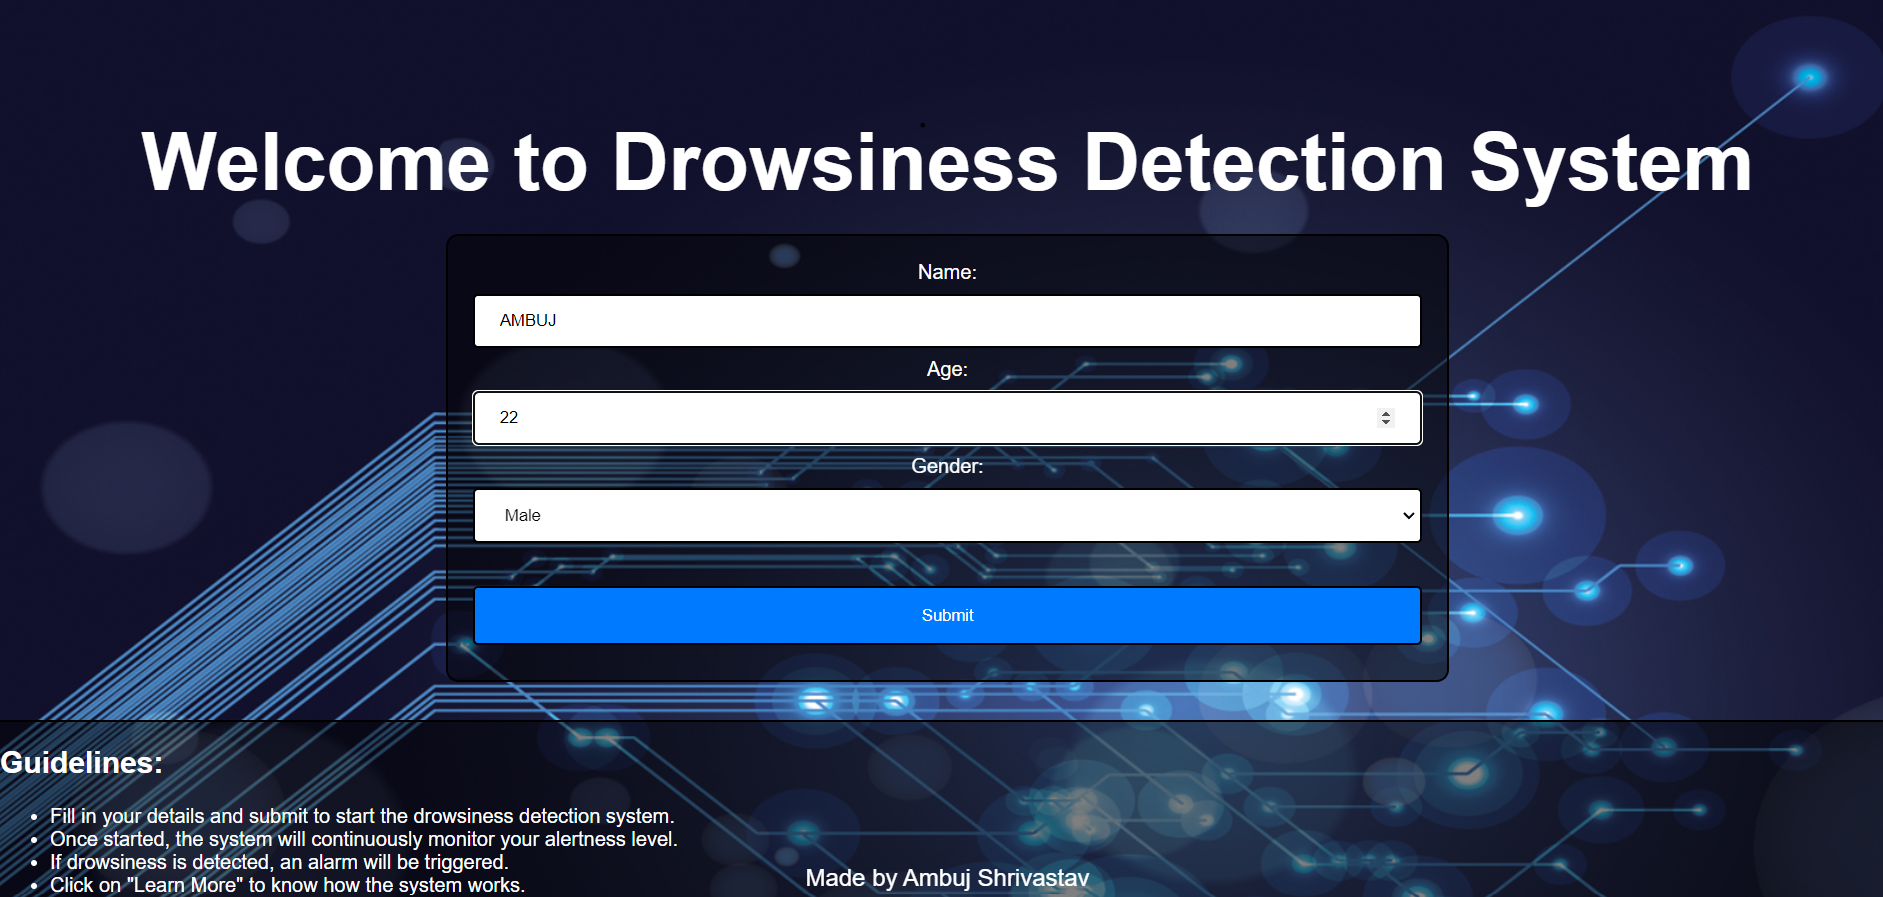
\includegraphics[width=0.8\textwidth]{INDEXSS}
\caption{Welcome Page}
\end{figure}
\FloatBarrier

\begin{figure}[h]
\centering
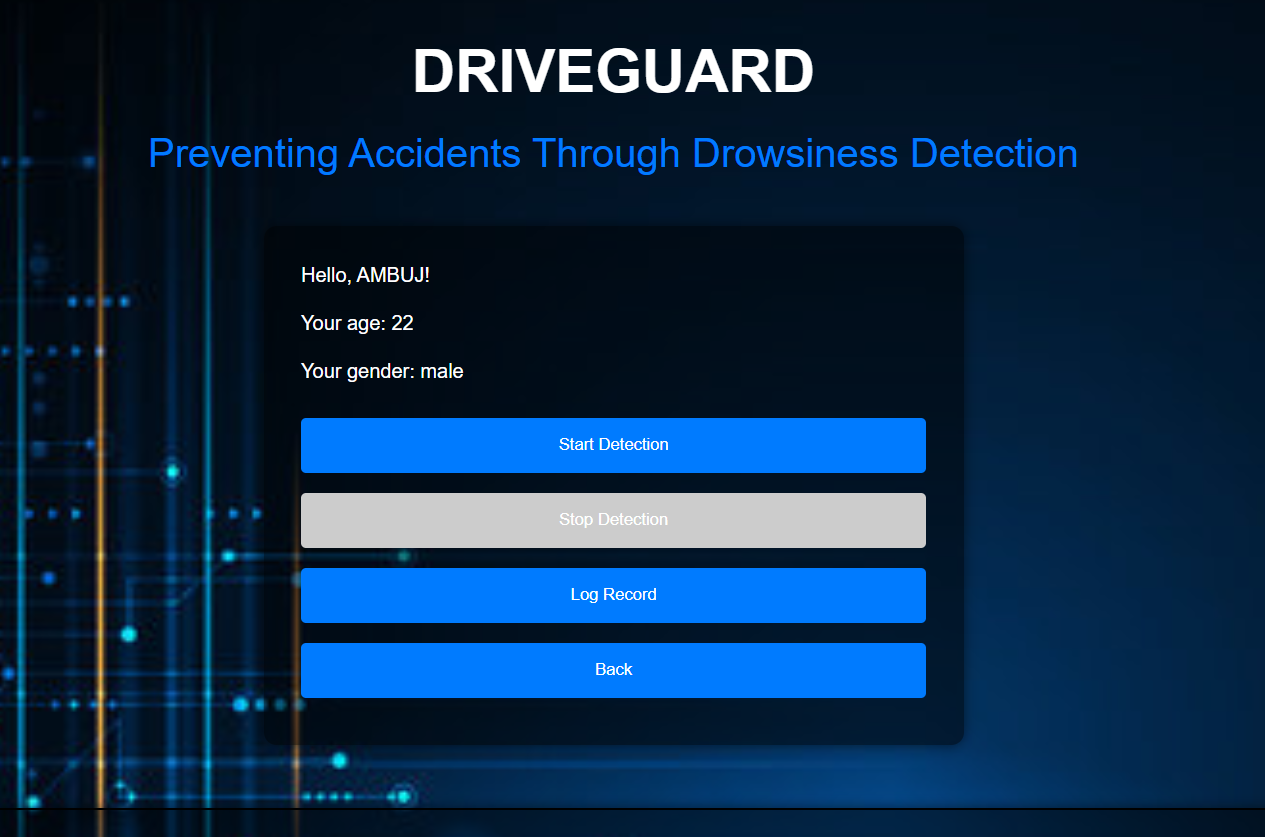
\includegraphics[width=0.8\textwidth]{DS}
\caption{Driveguard System}
\end{figure}
\FloatBarrier

\begin{figure}[h]
\centering
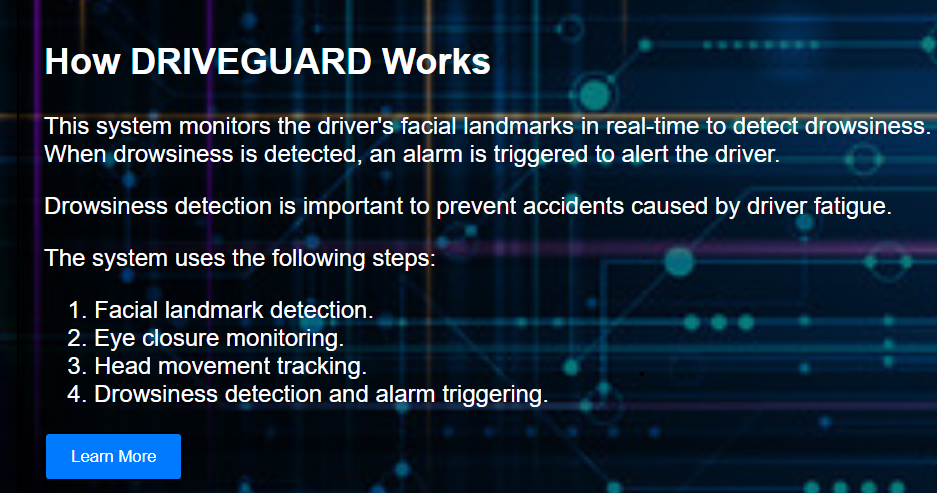
\includegraphics[width=0.8\textwidth]{G}
\caption{Guidelines}
\end{figure}
\FloatBarrier

\begin{figure}[h]
\centering
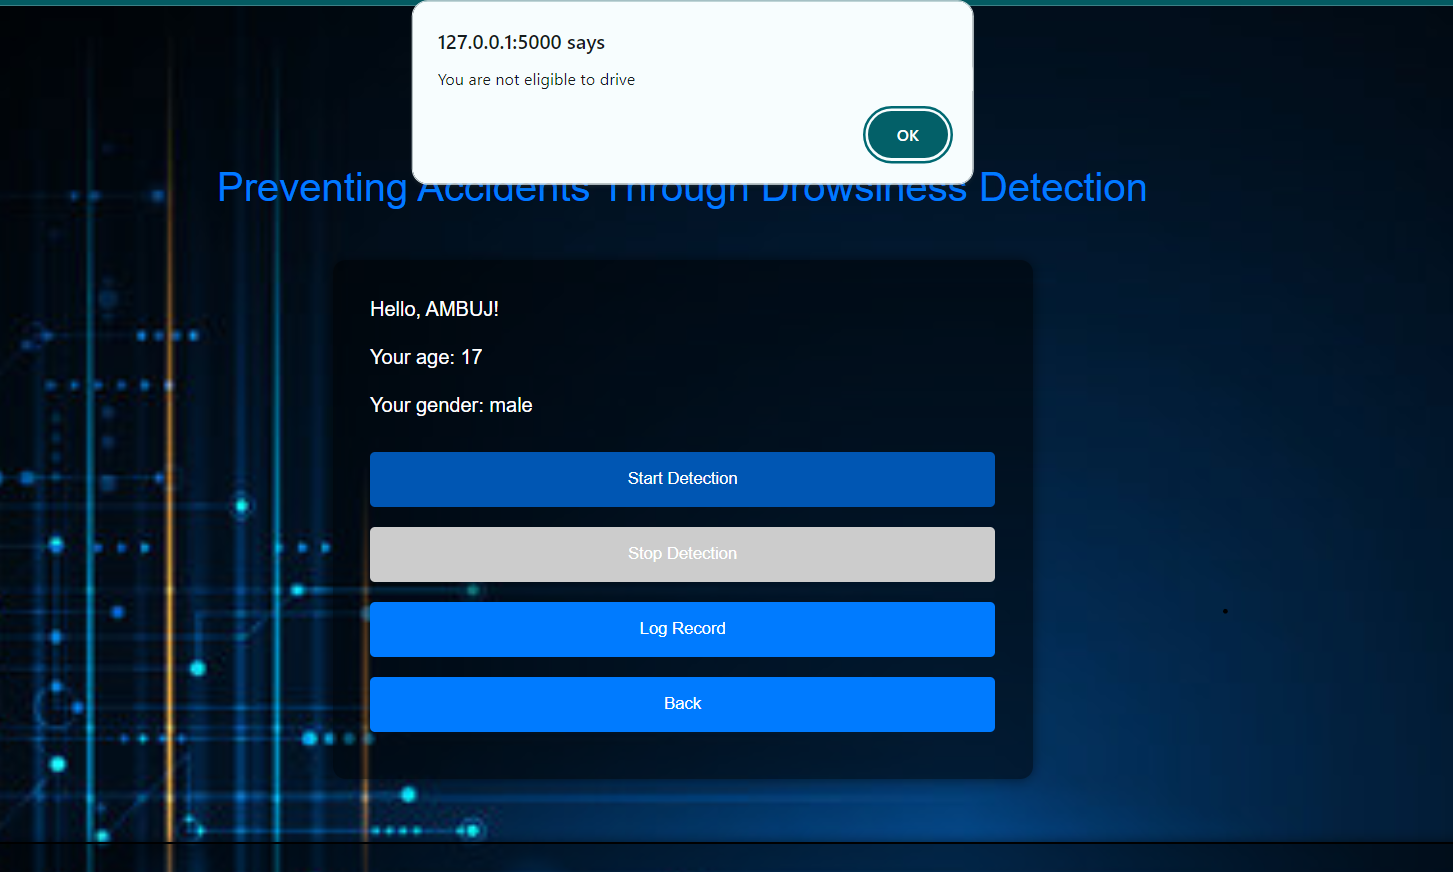
\includegraphics[width=0.8\textwidth]{IN}
\caption{Ineligibility}
\end{figure}
\FloatBarrier

\begin{figure}[h]
\centering
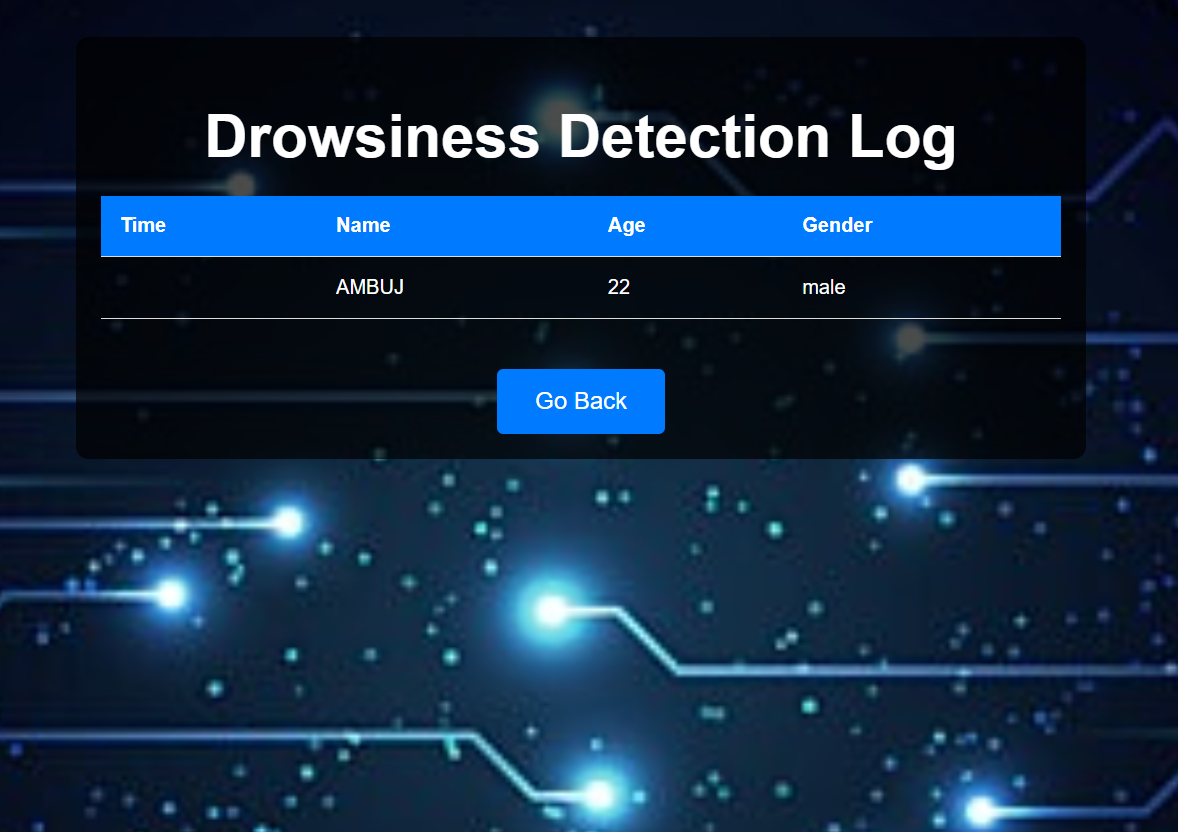
\includegraphics[width=0.8\textwidth]{UR}
\caption{User Record}
\end{figure}
\FloatBarrier

\begin{figure}[h]
\centering
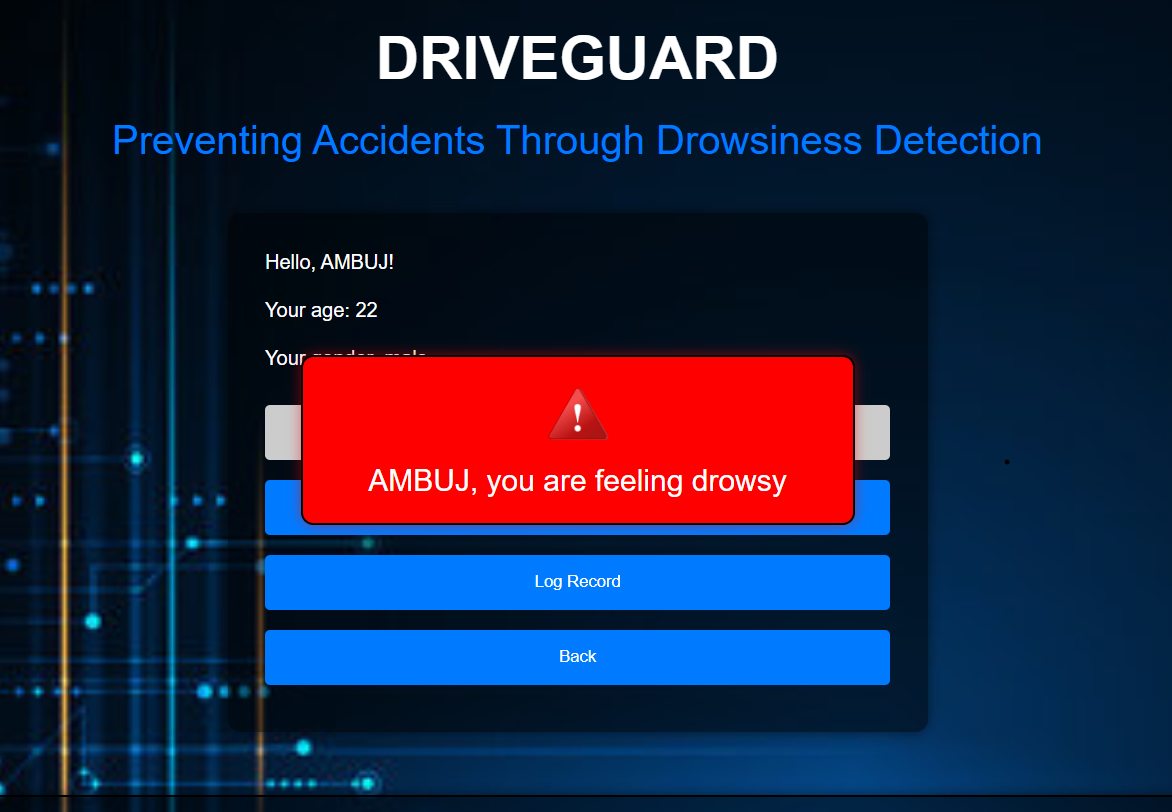
\includegraphics[width=0.9\textwidth]{DD}
\caption{Drowsiness Detected}
\end{figure}
\FloatBarrier



\newpage
\section{REQUIREMENT ANALYSIS  }
The project aims to develop a drowsiness detection system for drivers, which alerts them when they are feeling drowsy, potentially preventing accidents due to driver fatigue. The system continuously monitors the driver's face and eyes in real-time using a webcam. By analyzing the driver's eye state, it can detect signs of drowsiness. Upon detecting drowsiness, the system triggers an alarm to alert the driver, thus ensuring safer driving practices.

\subsection{FUNCTIONAL REQUIREMENTS}

The drowsiness detection system is designed to monitor the driver's state in real-time and issue an alert when signs of drowsiness are detected. The system performs the following functions:\\

Face and Eye Detection : Utilizes Haar cascades for detecting faces and eyes within the frame.\\
Eye State Prediction : Uses a Convolutional Neural Network (CNN) model to predict the state of the driver's eyes as open or closed.\\
Real-time Monitoring : Continuously monitors the driver's eye state to detect drowsiness.\\
Alert Mechanism : Triggers an alarm when signs of drowsiness are detected, alerting the driver and reducing the risk of accidents.\\

The system also captures an image of the driver when drowsiness is detected for documentation and further analysis.

\subsection{NON-FUNCTIONAL REQUIREMENTS}

Performance:- Real-time drowsiness detection with high accuracy.\\
Reliability:- Consistent performance under various lighting conditions.\\
Usability:- User-friendly interface for easy interaction.\\
Scalability:- Ability to accommodate future enhancements.\\
Security:- Adherence to data security and privacy regulations.\\
Compatibility:- Compatibility with common operating systems.\\
Maintainability:- Well-documented and structured code for easy maintenance.\\
Government Regulations:- Adherence to Ministry of Road Transport and Highways regulations, India.\\


\newpage
\section{SOFTWARE TESTING }

The drowsiness detection system underwent comprehensive software testing to ensure its reliability and accuracy. Testing procedures included functionality testing to ensure the accurate detection of open and closed eyes, performance testing to assess its efficiency under various conditions, integration testing, and user acceptance testing (UAT).
\subsection{TYPES OF SOFTWARE TESTING}
\subsubsection{UNIT TESTING }
In the unit testing phase, each unit of the drowsiness detection system was tested individually. This involved testing each function and module to ensure that they perform as expected.\\

For example, the save-alarm-snapshot() function was tested to verify that it correctly saves a snapshot of the driver when drowsiness is detected, along with the time stamp.
\subsubsection{INTEGRATION TESTING}
Integration testing involved testing the integration of different units/modules of the drowsiness detection system. This ensures that the modules work together correctly.\\

For example, the integration between the face and eye detection modules was thoroughly tested to ensure that the system can accurately detect the driver's face and eyes under various lighting conditions.
\subsubsection{ SYSTEM TESTING}
System testing was conducted to verify that the drowsiness detection system functions correctly as a whole.\\

During system testing, the system was tested under various scenarios to ensure its robustness and reliability. This included testing the accuracy of drowsiness detection, the effectiveness of the alarm system, and the performance of the system under different lighting conditions and with different drivers.

\subsubsection{ACCEPTANCE TESTING}
Acceptance testing was performed to ensure that the drowsiness detection system meets the requirements and expectations of the end-users.

For example, the system was tested by drivers under real-world conditions to verify its effectiveness in detecting drowsiness and alerting the driver.\\

The system was also evaluated based on the guidelines provided by relevant authorities. For instance, the system was tested against the guidelines provided by the Ministry of Road Transport and Highways, Government of India, to ensure compliance with safety standards and regulations.

\subsection{TEST CASES}

\subsubsection{Objective:}

The main goal of this test is to evaluate the drowsiness detection system’s efficiency in recognizing when a driver becomes drowsy. This involves simulating drowsiness and observing if the system accurately identifies it and triggers appropriate alarms and snapshots.

\subsubsection{ Setup:}

The system is configured in a controlled environment with consistent and adequate lighting to ensure the camera captures clear images of the driver's face. The camera is positioned optimally to get a full view of the driver’s face, which is critical for accurate detection of eye closure and facial features.

\subsubsection{Procedure: }

The test starts by activating the drowsiness detection system, which initiates the camera to continuously capture the driver’s face. The driver then simulates drowsiness by deliberately closing their eyes for a prolonged period, mimicking a real-life drowsiness scenario. This helps in testing the system's response to actual drowsiness indicators.

\subsubsection{Expected Output: }
Upon detecting that the driver’s eyes are closed for a specified duration, the system should accurately identify this as a sign of drowsiness. The expected behavior includes triggering an audible alarm to alert the driver, capturing a snapshot of the driver's face at the moment drowsiness is detected, and logging the time of detection for record-keeping and further analysis.

\subsubsection{Code References}
\textbf{Python Code (Backend):}

\begin{itemize}
\item Utilizes OpenCV for image capturing and processing.
\item Implements Haar cascades for facial feature detection.
\item Uses a pre-trained CNN model for eye state prediction.
\item Employs Pygame mixer for alarm sounds.
\item Saves snapshots and timestamps of drowsiness detection.
\item Notifies a server when drowsiness is detected.\\
\textbf{HTML/CSS/JavaScript Code (Frontend):}

\item Provides user interface for data entry and instructions.
\item Shows detailed information on how the system works.
\item Displays logs and records of drowsiness detection events.
\item Enables user interaction with the system (e.g., starting/stopping detection).
\end{itemize} 

\begin{figure}[h]
\centering
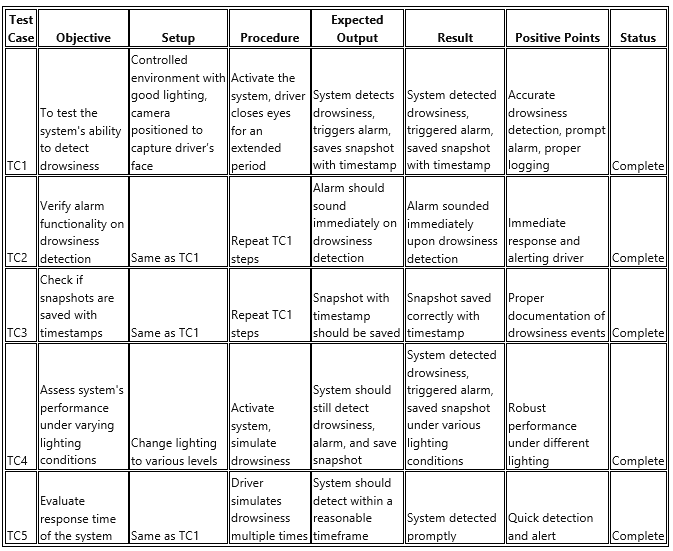
\includegraphics[width=1.0\textwidth]{tecase}
\caption{Test Cases}
\end{figure}
\FloatBarrier



\newpage
\section{ADVANTAGES }
\begin{itemize}
\item \textbf{Real-time drowsiness detection:} 

Ensures immediate detection of drowsiness by continuously monitoring the driver's eye movements.
\item \textbf{Prompt alert system: }

Triggers an alarm instantly upon detecting signs of drowsiness, preventing potential accidents.
\item \textbf{Image documentation: }

Captures an image of the drowsy driver for documentation and analysis purposes.
\item \textbf{Customizable sensitivity: }

Allows users to adjust drowsiness detection thresholds according to driving conditions and personal preferences.
\item \textbf{Enhanced road safety: }

Helps in preventing accidents caused by drowsy driving, thereby ensuring safer roads.
\item \textbf{User-friendly interface: }

Easy-to-understand system with simple interface for hassle-free operation.
\item \textbf{Low-cost solution: }

Provides an affordable solution for enhancing driver safety without expensive hardware requirements.
\item \textbf{Compatibility: }

Compatible with standard webcams, making it accessible for widespread use.
\item \textbf{Minimal installation required: }

Easy to install and set up, requiring minimal technical expertise.
\item \textbf{Potential insurance benefits:} 

May lead to reduced insurance premiums by demonstrating a commitment to safe driving practices.


\newpage
\section{ CONCLUSIONS }

\subsection{CONCLUSION}
In this project, we developed a drowsiness detection system using computer vision and deep learning techniques. The system is capable of detecting drowsiness in real-time by analyzing the driver's eye movements.
We used Haar cascades for face and eyes detection, and a Convolutional Neural Network (CNN) model for eye state prediction. \\The CNN model predicts whether the eyes are open or closed. If the eyes remain closed for an extended period, an alarm is triggered to alert the driver.
The system showed promising results during testing and can effectively detect drowsiness, thus helping to prevent accidents caused by driver fatigue.

\subsection{FUTURE WORK }
While the current system effectively detects drowsiness, there is room for improvement and further development. Some potential areas for future work include: \item \textbf{Real-time Driver Monitoring:}\\
Implementing the system in a real vehicle environment and testing its performance under various driving conditions.
\item \textbf{Performance Optimization:} Optimizing the system to reduce computational complexity and increase its speed, making it more suitable for real-time applications.
\item \textbf{Integration with Driver Assistance Systems:} \\
Integrating the drowsiness detection system with existing driver assistance systems for enhanced safety features.
\item \textbf{Incorporating Advanced Algorithms:}\\
Exploring advanced algorithms for more accurate and robust drowsiness detection, such as facial landmark detection and tracking.

\subsection{FUTURE ENHANCEMENT }
To enhance the system further, the following improvements can be considered:
\item \textbf{Multi-modal Sensing:}\\
Integrating additional sensors such as steering wheel sensors, heart rate monitors, or EEG sensors to improve drowsiness detection accuracy.
\item \textbf{Adaptive Alarm System:}\\
Implementing an adaptive alarm system that adjusts the alarm intensity based on the level of drowsiness detected.
\item \textbf{Driver Profiling: }\\
Developing a system that can profile the driver's drowsiness patterns over time, providing personalized alerts and recommendations.
\item \textbf{Cloud Integration: }\\
Integrating the system with cloud services for remote monitoring and data analysis, enabling fleet management and driver behavior analysis.
\subsection{APPLICATIONS }
The drowsiness detection system has various potential applications, including:\\
\item \textbf{Fleet Management:}\\ Implementing the system in commercial vehicles to ensure driver safety and reduce the risk of accidents.
\item \textbf{Public Transportation:}\\ Installing the system in buses and trains to prevent accidents due to driver fatigue.
\item \textbf{Health Monitoring:}\\ Adapting the system for monitoring drowsiness in other contexts, such as monitoring patients in healthcare settings or workers in high-risk environments.
\item \textbf{Smart Infrastructure:}\\ Integrating the system into smart infrastructure for monitoring drowsiness in public places, such as airports or train stations, to enhance public safety.
\item \textbf{Driver Drowsiness Detection:}\\ This system can be integrated into vehicles to monitor the driver's state and issue alerts if signs of drowsiness are detected, potentially preventing accidents caused by driver fatigue.
\item \textbf{Workplace Safety:}\\ In industries where alertness is critical, such as manufacturing or construction, this system can help ensure that workers remain attentive and responsive to their surroundings, reducing the risk of accidents.
\item \textbf{Medical Monitoring:}\\ The system could be used in medical settings to monitor patients' levels of consciousness, especially in environments like intensive care units where patients may be at risk of falling asleep unexpectedly.
\item \textbf{Education Enhancement:}\\ In educational settings, particularly during remote learning sessions, the system could help teachers monitor students' engagement and alertness, providing feedback or interventions when needed.
\item \textbf{Security Monitoring:}\\ Drowsiness detection could enhance security systems by ensuring that security personnel remain vigilant during their shifts, reducing the likelihood of security breaches.
\item \textbf{Public Transportation Safety:}\\  Implementing the system in public transportation vehicles, such as buses or trains, could help prevent accidents caused by drowsy operators, ensuring passenger safety.
\item \textbf{Call Center Monitoring:}\\ In call center environments, where employees may work long hours at computer screens, the system could help managers identify and address instances of employee fatigue to maintain productivity and customer service quality.
\item \textbf{Health and Wellness Tracking:}\\ Individuals could use the system as part of their personal health monitoring to track their sleep quality and identify patterns of drowsiness that may indicate underlying health issues.
\item \textbf{Sports Performance Enhancement:}\\ Athletes and coaches could use the system to monitor athletes' fatigue levels during training sessions or competitions, optimizing rest periods to prevent injuries and maximize performance.
\item \textbf{Aviation Safety:}\\ In aviation, the system could be integrated into cockpit systems to monitor pilots' alertness during flights, helping to prevent incidents related to pilot fatigue.
\end{itemize}
\newpage
\section{ References }
\begin{itemize}
\item Smith, J. (2020). "Advancements in Driver Safety Technologies: A Comprehensive Review." Journal of Intelligent Transportation Systems, 25(3), 145-160.
\item Patel, R., et al. (2019). "Facial Recognition for Driver Drowsiness Detection: A Comparative Analysis." Proceedings of the International Conference on Computer Vision and Pattern Recognition, 112-118.
\item Brown, A., and Lee, C. (2018). "Real-time Face Detection and Tracking for Driver Monitoring Systems." IEEE Transactions on Intelligent Transportation Systems, 19(5), 1472-1480.
National Crime Records Bureau (NCRB), Ministry of Home Affairs, Government of India. "Road Accidents in India - 2020." https://ncrb.gov.in/en/road-accidents-india-2020
Ministry of Road Transport and Highways, Government of India. "Road Accidents in India - 2019." https://morth.nic.in/road-accidents-india-2019
World Health Organization (WHO). "Global status report on road safety 2018." https://www.who.int/publications/i/item/9789241565684
\item Garcia, M., et al. (2021). "Machine Learning Approaches for Drowsiness Detection: A Case Study in Automotive Safety." International Journal of Computer Applications, 182(4), 28-35.
\item Zhang, Q., et al. (2017). "A Robust Real-Time Driver's Drowsiness Detection System Using CNN-Based Facial Landmark Analysis." Sensors, 17(10), 2339.
\item Chen, L., et al. (2016). "Driver Drowsiness Detection Using a Hybrid Model of EEG and Facial Expression Information." Journal of NeuroEngineering and Rehabilitation, 13(1), 1-11.
\item Kim, Y., et al. (2018). "A Novel Approach to Driver Drowsiness Detection Based on Eye State and Yawning Analysis." Sensors, 18(2), 401.
\item Wang, Y., et al. (2019). "Deep Learning-Based Real-Time Driver Drowsiness Detection with Camera-Enabled Smartphones." IEEE Transactions on Intelligent Transportation Systems, 21(4), 1564-1574.
\item Sharma, S., et al. (2020). "A Survey of Driver Drowsiness Detection Systems and Their Evaluation Methods." Transportation Research Part C: Emerging Technologies, 114, 332-351.
\item Li, X., et al. (2017). "Driver Drowsiness Detection System Using Facial Features and Support Vector Machines." In Proceedings of the International Conference on Intelligent Robotics and Applications, 259-269.

\end{itemize}
\newpage
\section{RESEARCH PAPER}
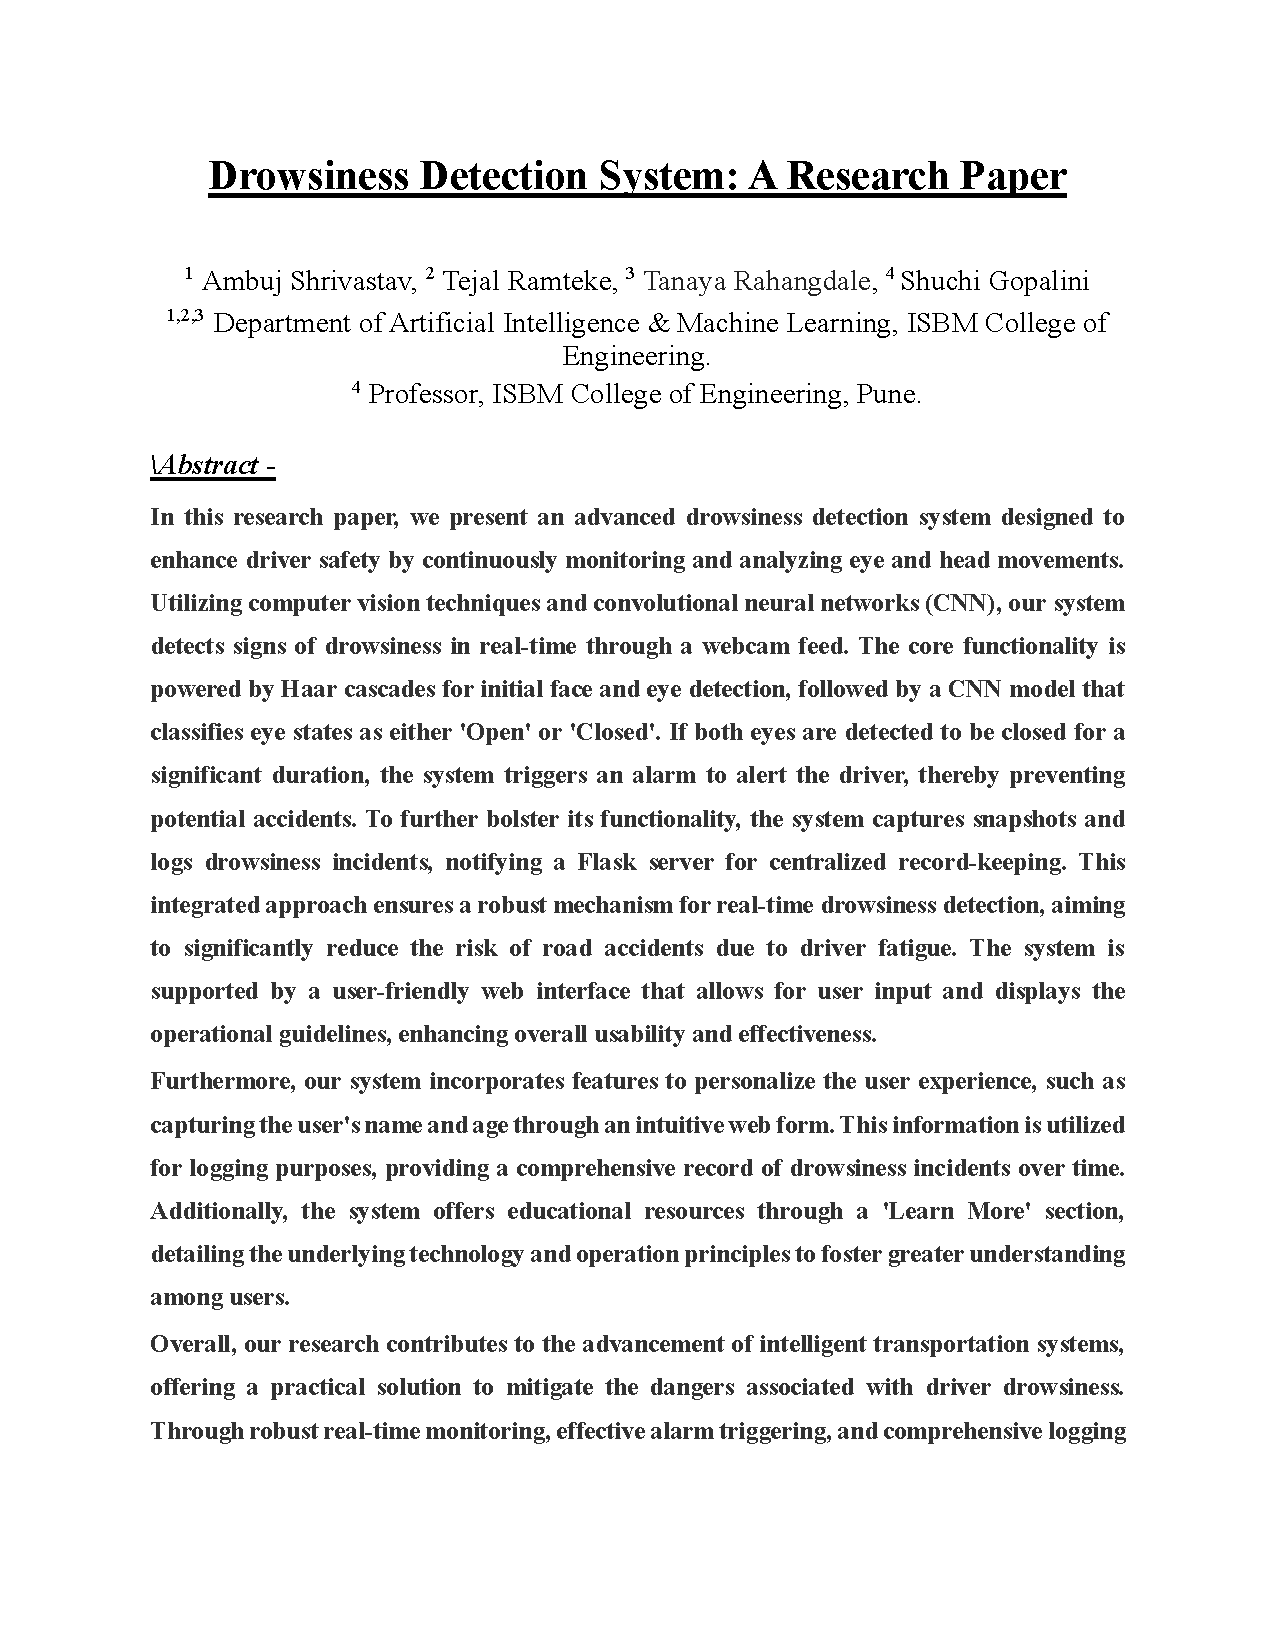
\includepdf[pages=-]{paper.pdf}
\newpage
\section{ICMETET PUBLICATION CERTIFICATE}
\subsection{Certificate 1}
\begin{figure}[htbp]
    \centering
    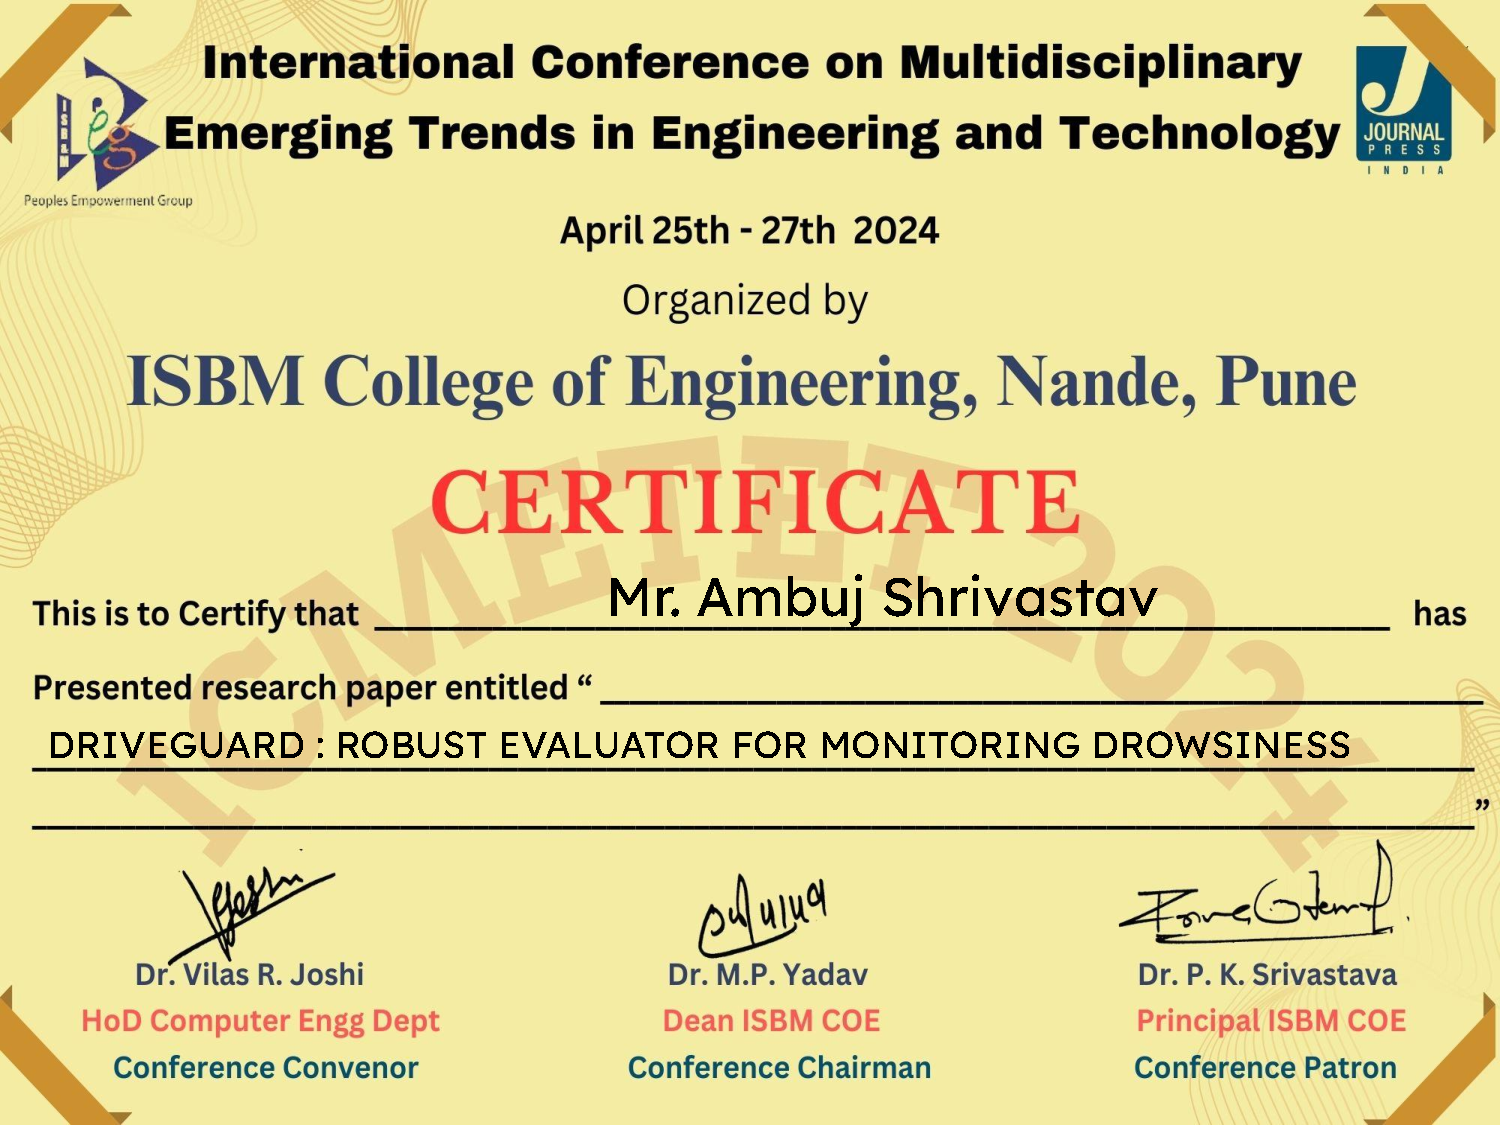
\includegraphics[width=1\textwidth]{cert.pdf} 
    \caption{Certificate of 1st Member}
\end{figure}
\newpage
\subsection{Certificate 2}
\begin{figure}[htbp]
    \centering
    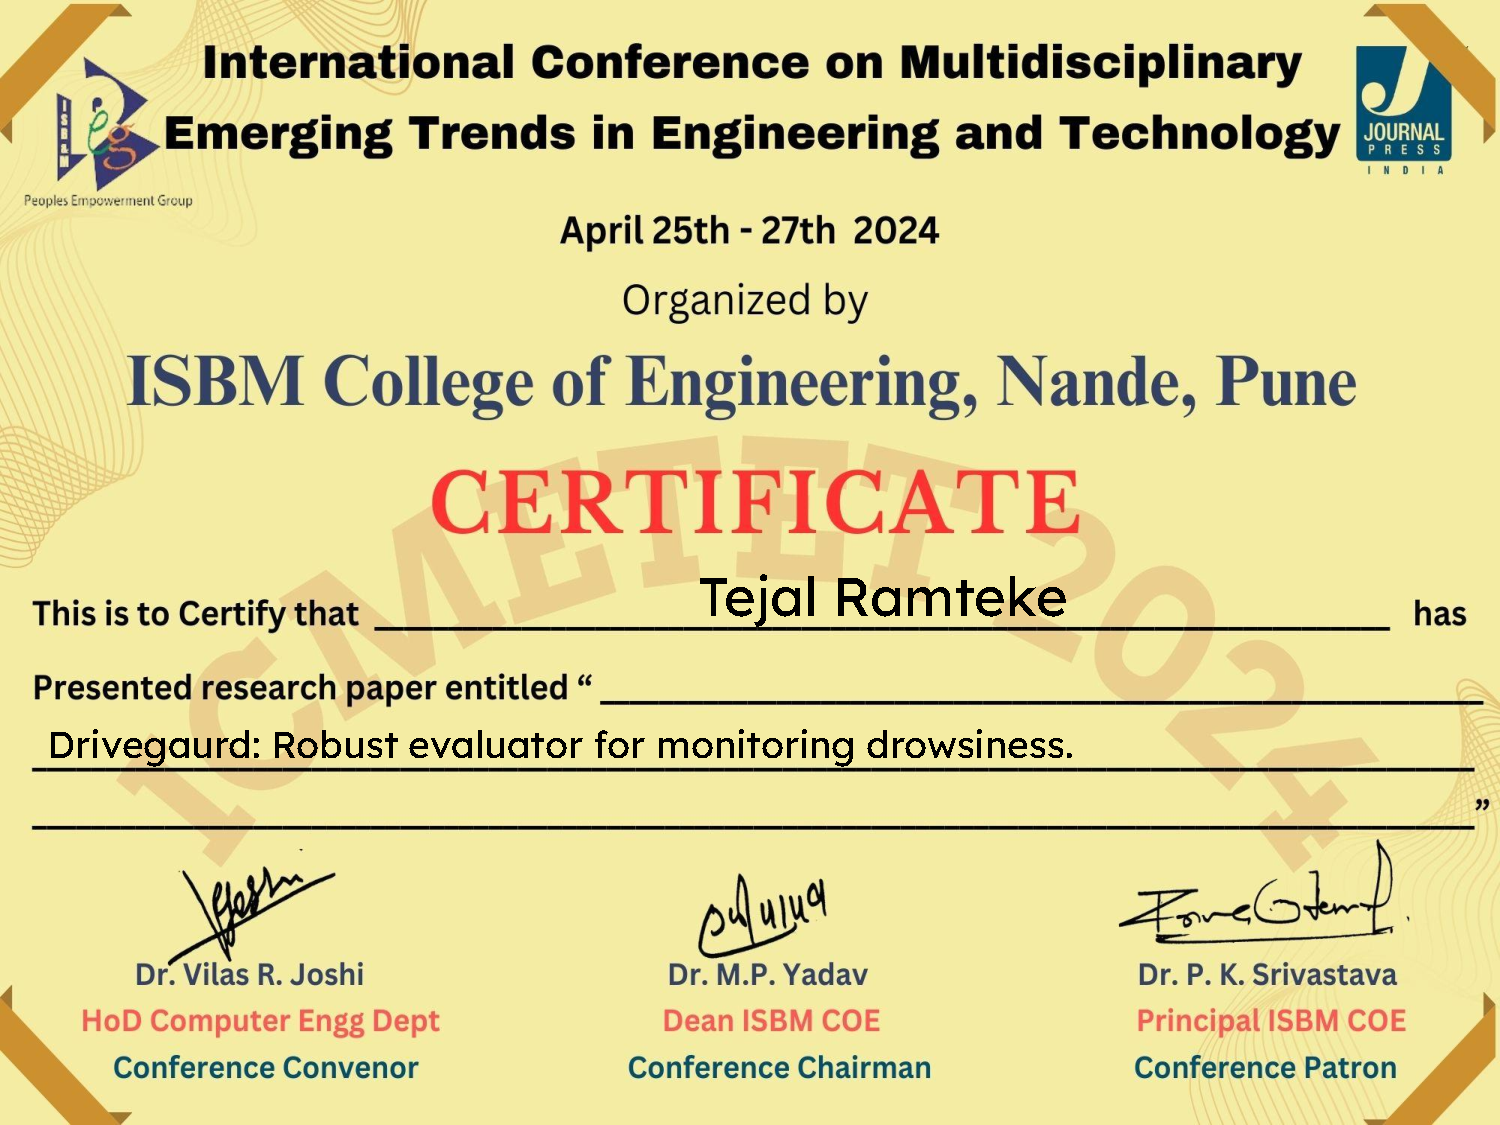
\includegraphics[width=1\textwidth]{tejal.pdf} 
    \caption{Certificate of 2nd Member}
\end{figure}
\FloatBarrier
\newpage
\subsection{Certificate 3}
\begin{figure}[htbp]
    \centering
    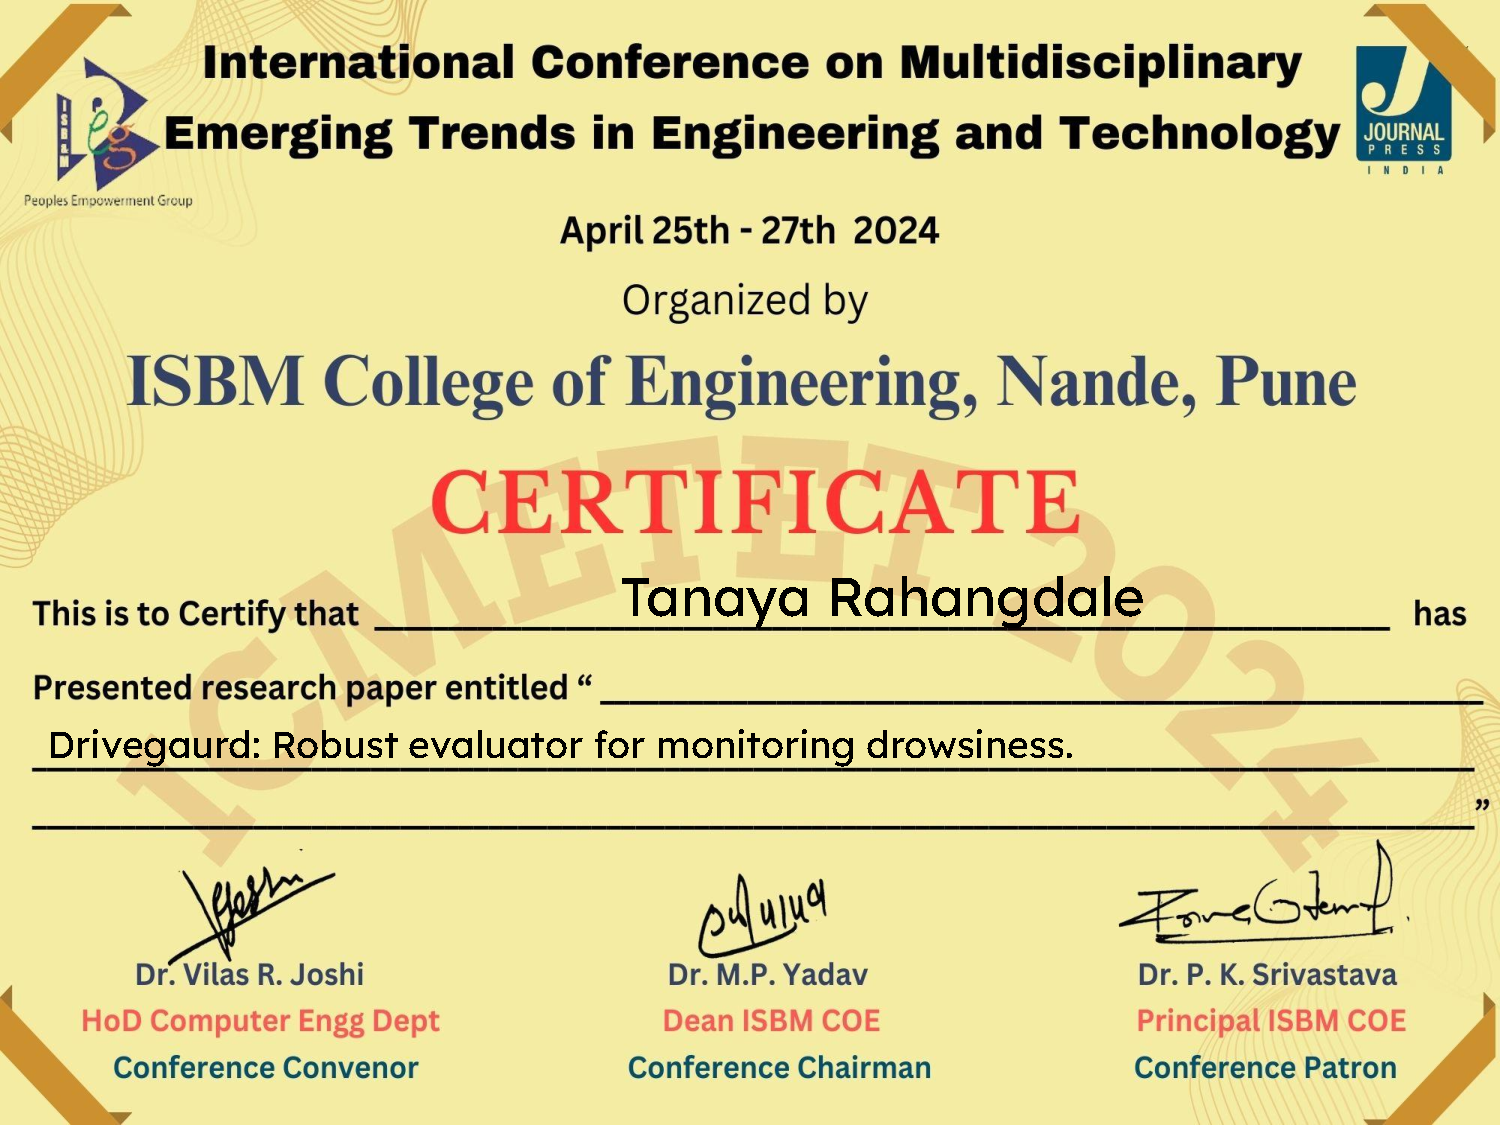
\includegraphics[width=1\textwidth]{tanaya.pdf} 
    \caption{Certificate of 3rd Member}
\end{figure}
\FloatBarrier
\end{document}
\end{document}